% File tacl2021v1.tex
% Dec. 15, 2021

% The English content of this file was modified from various *ACL instructions
% by Lillian Lee and Kristina Toutanova
%
% LaTeXery is mostly all adapted from acl2018.sty.

\documentclass[11pt,a4paper]{article}
\usepackage{times,latexsym}
\usepackage{url}
\usepackage[T1]{fontenc}

\usepackage{graphicx} 
\usepackage{multirow}

\usepackage{caption}
\usepackage{subcaption}

\usepackage{amsmath}
\usepackage{makecell}

\usepackage{hyperref}

\usepackage{comment}

\usepackage{enumitem}




%% Package options:
%% Short version: "hyperref" and "submission" are the defaults.
%% More verbose version:
%% Most compact command to produce a submission version with hyperref enabled
%%    \usepackage[]{tacl2021v1}
%% Most compact command to produce a "camera-ready" version
%%    \usepackage[acceptedWithA]{tacl2021v1}
%% Most compact command to produce a double-spaced copy-editor's version
%%    \usepackage[acceptedWithA,copyedit]{tacl2021v1}
%
%% If you need to disable hyperref in any of the above settings (see Section
%% "LaTeX files") in the TACL instructions), add ",nohyperref" in the square
%% brackets. (The comma is a delimiter in case there are multiple options specified.)

\usepackage[acceptedWithA]{tacl2021v1}
%\usepackage{tacl2021v1}
% \setlength\titlebox{10cm} % <- for Option 2 below

%%%% Material in this block is specific to generating TACL instructions
\usepackage{xspace,mfirstuc,tabulary}


\usepackage{booktabs}

\newcommand{\dateOfLastUpdate}{Dec. 15, 2021}
\newcommand{\styleFileVersion}{tacl2021v1}

\newcommand{\ex}[1]{{\sf #1}}

\newif\iftaclinstructions
\taclinstructionsfalse % AUTHORS: do NOT set this to true
\iftaclinstructions
\renewcommand{\confidential}{}
\renewcommand{\anonsubtext}{(No author info supplied here, for consistency with
TACL-submission anonymization requirements)}
\newcommand{\instr}
\fi

%
\iftaclpubformat % this "if" is set by the choice of options
\newcommand{\taclpaper}{final version\xspace}
\newcommand{\taclpapers}{final versions\xspace}
\newcommand{\Taclpaper}{Final version\xspace}
\newcommand{\Taclpapers}{Final versions\xspace}
\newcommand{\TaclPapers}{Final Versions\xspace}
\else
\newcommand{\taclpaper}{submission\xspace}
\newcommand{\taclpapers}{{\taclpaper}s\xspace}
\newcommand{\Taclpaper}{Submission\xspace}
\newcommand{\Taclpapers}{{\Taclpaper}s\xspace}
\newcommand{\TaclPapers}{Submissions\xspace}
\fi

%%%% End TACL-instructions-specific macro block
%%%%

\title{Benchmarking Linguistic Diversity of Large Language Models}

% Author information does not appear in the pdf unless the "acceptedWithA" option is given

% The author block may be formatted in one of two ways:

% Option 1. Author’s address is underneath each name, centered.

\author{
  Yanzhu Guo\Thanks{This work was partially done during the author's affiliation with École Polytechnique.} 
  \\
  ALMAnaCH
  \\
  Inria Paris
  \And
  Guokan Shang
  \\
  France Lab
  \\
  MBZUAI\\
  \texttt{yanzhu.guo@inria.fr}\\
  \texttt{guokan.shang@mbzuai.ac.ae}\\
  \texttt{chloe.clavel@inria.fr}
  \And
  Chloé Clavel
  \\
  ALMAnaCH
  \\
  Inria Paris
}

% % Option 2.  Author’s address is linked with superscript
% % characters to its name, author names are grouped, centered.

% \author{
%   Template Author1\Thanks{The {\em actual} contributors to this instruction
%     document and corresponding template file are given in Section
%     \ref{sec:contributors}.}$^\diamond$ 
%   \and
%   Template Author2$^\dagger$
%   \\
%   \ \\
%   $^\diamond$Template Affiliation1/Address Line 1
%   \\
%   Template Affiliation1/Address Line 2
%   \\
%   Template Affiliation1/Address Line 2
%   \\
%   \texttt{template.email1example.com}
%   \\
%   \ \\
%   \\
%   $^\dagger$Template Affiliation2/Address Line 1
%   \\
%   Template Affiliation2/Address Line 2
%   \\
%   Template Affiliation2/Address Line 2
%   \\
%   \texttt{template.email2@example.com}
% }

\date{}

\begin{document}
\maketitle
\begin{abstract}
The development and evaluation of Large Language Models (LLMs) has primarily focused on their task-solving capabilities, with recent models even surpassing human performance in some areas. However, this focus often neglects whether machine-generated language matches the human level of diversity, in terms of vocabulary choice, syntactic construction, and expression of meaning, raising questions about whether the fundamentals of language generation have been fully addressed.
This paper emphasizes the importance of examining the preservation of human linguistic richness by language models, given the concerning surge in online content produced or aided by LLMs.
We propose a comprehensive framework for evaluating LLMs from various linguistic diversity perspectives including lexical, syntactic, and semantic dimensions. Using this framework, we benchmark several state-of-the-art LLMs across all diversity dimensions, and conduct an in-depth case study for syntactic diversity. Finally, we analyze how different development and deployment choices impact the linguistic diversity of LLM outputs.


\end{abstract}

\section{Introduction}

%to do: formalize the problem (define a function), empahsize that we are analyzing linguistic diversity at a macro level. LLM outputs at scale. Different from evaluating diversity output of a single human.

Recent Large Language Models (LLMs) have exhibited outstanding capabilities in generating both natural and formal language \citep{brown2020language, touvron2023llama}, while also achieving human-level performance in language understanding, commonsense reasoning, and various other tasks \citep{hendrycks2020measuring}. This has led to evaluations that predominantly focus on these specific abilities \citep{wang2024mmlu}. Meanwhile, other evaluation studies address well-recognized issues in LLMs, such as factuality \citep{maynez-etal-2020-faithfulness}, safety \citep{zhang-etal-2024-safetybench}, and fairness \citep{gallegos-etal-2024-bias}, which remain focal points of ongoing research.
However, there is a notable lack of attention paid to linguistic perspectives, particularly in diversity \citep{guo-etal-2024-curious}, despite the fundamental objective of natural language generation being to produce outputs that are not only \textit{accurate} but also \textit{diverse} \citep{tevet-berant-2021-evaluating}.
%\citep{rawte-etal-2023-troubling}
%arithmetic reasoning \citep{imani-etal-2023-mathprompter}
%We can define linguistic diversity as the condition of human language as composed of different registers and dialects, which are all linguistically equal but socially differentiated, in other words, equally rule-governed and responsive to community needs but valued differently according to socially constructed hierarchies and represented unequally in collectable data \citep{aulllanguage}. For example, a large portion of pretraining data from the web comes from wikipedia pages, which are based on the norms of a single dialect, standardized written academic English.
%Linguistic diversity refers to the variety within human language, including different registers and dialects. These variations are linguistically equal, though each is governed by specific rules, but socially differentiated to be responsive to community needs \citep{aulllanguage}.

%In this paper, we define linguistic diversity as the inherent variation within human language, encompassing vocabulary usage, grammatical structures, and semantic nuances. This diversity is crucial for capturing and preserving the richness of human language \citep{aulllanguage}.

%, yet valued differently due to social hierarchies and unequal representation in collectable data \citep{aulllanguage}.
%For instance, a large portion of pretraining data from the web comes from Wikipedia pages, which adhere to the norms of a single dialect: standardized written academic English.
%Therefore, linguistic diversity plays a role in reflecting and preserving cultural richness, and when two language models achieve the same functional purposes, the one generating more diverse language should be deemed more desirable.
%Therefore, linguistic diversity plays a role in reflecting and preserving cultural richness, making a model generating more diverse language more desirable among those that achieve the same functional purposes.
%Human expressions are full of nuances and variations that current models often fail to fully capture, as studies comparing human and model-generated content have shown \citep{guo-etal-2024-curious,shaib2024standardizing,giulianelli-etal-2023-comes}.

%Recent research has raised concerns about the linguistic diversity of LLM outputs by drawing comparisons between human and model-generated content, which revealed that models often fail to capture the nuances and variations in human expressions \citep{shaib2024standardizing,giulianelli-etal-2023-comes}. These concerns extend to findings that training language models on synthetic text causes a decline of diversity \citep{guo-etal-2024-curious}.

Recent studies have highlighted concerns regarding the linguistic diversity of LLM outputs. By comparing human and model-generated content, researchers have shown that models frequently struggle to reflect the nuances and variations characteristic of human expression \citep{shaib2024standardizing,giulianelli-etal-2023-comes}. Additionally, these concerns are reinforced by findings that training language models on synthetic text can lead to a further decline in linguistic diversity \citep{guo-etal-2024-curious}.

In fact, LLMs tend to be inherently conservative in producing diverse content. During training, models undergo homogenization to the most frequent patterns in the training data, where creative outlier narratives, views, styles, and knowledge are often underrepresented \citep{kandpal2023large}. Unlike models, human language production involves a complex interplay of factors that go beyond merely optimizing probabilities \citep{Holtzman2020The}. It is therefore crucial to emphasize evaluating output diversity in language models and systematically consider these metrics to guide future model development and deployment decisions.

%As previously said, the increasing recognition and use of LLMs in society have led to a significant rise in online content produced or assisted by these models \citep{geng2024chatgpt}. Examining whether LLMs can preserve human linguistic richness has hence become increasingly important.
Currently, a principled and comprehensive evaluation framework for linguistic diversity is lacking in the literature \citep{shaib2024standardizing}.	
While some studies on Natural Language Generation (NLG) report diversity metrics, they typically focus on a single diversity aspect (e.g., lexical diversity~\citep{chakrabarty-etal-2022-help}), often experimenting within a single domain and task (e.g., news summarization ~\citep{shaib2024standardizing}). This narrow focus is problematic since diversity varies across aspects and depends on the domain \citep{guo-etal-2024-curious}.	
Although some efforts have been made to assess the influence of reinforcement learning from human feedback (RLHF) on diversity \citep{kirk2024understanding}, the impact of other key design and development stages—such as model scale, quantization, and decoding strategy—remains unexplored. 
Additionally, there is a limited understanding of how LLMs develop the capability to generate diverse language through successive pretraining checkpoints.
Ultimately, no study has benchmarked the diversity performance of state-of-the-art LLMs across different aspects and domains.

% why linguistic diversity is important, for human, culture-wise, language
% why need to care about it for LLMs.
% relationships.
% if not, consequences:
% \citep{guo2023curious}

In this work, we first establish a framework for evaluating linguistic diversity of LLM outputs on a corpus level. We then benchmark six prominent LLMs on five NLG tasks, and compare the diversity of their outputs across three different aspects: lexical, syntactic, and semantic. We further explore syntactic diversity, and conduct a case study comparing the distribution of dependency trees generated by LLMs and humans. Finally, we investigate how LLM output diversity changes across different development stages, and with varying decisions of deployment.
The main research questions we address are as follows:	
\begin{enumerate}[noitemsep,topsep=0pt,parsep=0pt,partopsep=0pt,leftmargin=*]
    \item What are the key aspects of LLM output diversity, and how can they be evaluated? (See \textsection~\ref{sec:diversity})
    \item How do state-of-the-art LLMs perform in terms of diversity across different tasks? (See \textsection~\ref{sec:benchmarking_results})
    \item How does diversity change during each LLM development stage (e.g., pretraining, supervised fine-tuning (SFT), preference tuning)? (See \textsection~\ref{sec:training_stages})
    \item How do different design (e.g., model scale, training data) and deployment (e.g., decoding strategy, quantization) choices affect diversity?	(See \textsection~\ref{sec:decoding} and \textsection~\ref{sec:scale_quant})
\end{enumerate}

\noindent It is worth noting that we study linguistic diversity in a monolingual context, focusing on the English language. However, the evaluation methodology is language agnostic and could easily be extended to other languages, given that employed NLP toolkits (e.g., dependency parsers, sentence embeddings) exist for the language. Furthermore, our approach to analyzing the influence of various factors on LLM outputs is adaptable to other dimensions, such as linguistic naturalness \citep{guo2024large}.
The code is publicly available\footnote{\tiny\url{https://github.com/YanzhuGuo/llm-diversity}}.


\section{Related Work}
	
In this section, we review methods for evaluating and analyzing \textit{linguistic diversity}. We define linguistic diversity as the natural variation in human language across core linguistic properties, including vocabulary usage, grammatical structures, and semantic nuances. In contrast, a separate line of research focuses on \textit{socio-linguistic diversity} \citep{hayati2023far, lahoti-etal-2023-improving}, which falls beyond the scope of our study.

%which examines higher-level factors such as perspective \citep{hayati2023far} and cultural or demographic representation \citep{lahoti-etal-2023-improving}. These aspects, however, fall beyond the scope of our study.

%, which study core linguistic properties such as the vocabulary, syntax, and semantics.		
%In contrast, another line of research investigates \textit{socio-linguistic diversity}, focusing on higher-level factors such as perspective \citep{hayati2023far} or representation, including demographic and cultural aspects \citep{lahoti-etal-2023-improving}. These topics fall outside the scope of our study.

%We leave socio-linguistic diversity for future work.	


\subsection{Evaluation of Human Language} \label{subsec:human}
Early metrics for linguistic diversity, proposed by linguists, were developed for studies of language acquisition and language disorder detection. For example, \citet{fergadiotis2013measuring} employed lexical diversity metrics to identify symptoms of aphasia, while \citet{mcnamara2010linguistic} showed that both syntactic complexity and lexical diversity can predict essay quality.		
Another study by \citet{a89efe5d-217a-3260-b2b1-1437ae204234} manually annotated a small corpus of texts produced by second language learners for syntactic features such as syntactic length and clause types, considering their variation as a diversity index. 
However, these metrics are limited to evaluating human-written texts and either focus exclusively on lexical diversity or lack scalability due to the need for manual annotation.	

The evaluation of linguistic diversity in model-generated language has emerged as a relatively recent focus of research. This development is driven, in part, by growing concerns over the increasing prevalence of model-generated or model-influenced content online, prompting questions about whether LLMs can maintain the linguistic richness characteristic of human language \citep{guo-etal-2024-curious}. Moreover, advances in language generation quality have brought model outputs closer than ever to human-level coherence and plausibility. Assessing linguistic diversity becomes meaningful \textit{only when} the generated text meets these standards. For example, a randomly initialized model might produce token sequences with high lexical diversity, but such outputs hold no practical value \citep{uchendu2023does}.	

\smallskip

\subsection{Evaluation of Generated Language}
To the best of our knowledge, \citet{tevet-berant-2021-evaluating} were the first authors to systematically evaluate diversity in NLG.	
They proposed to create diversity metrics from any two-sentence similarity measure, defining diversity as the inverse of the mean similarity score across all unordered pairs.		
N-gram-based metrics were used to assess form diversity, while model-based metrics like Sentence-BERT similarity measured content diversity.		
They concluded that a notable disparity exists between automatic metrics and human judgment, and that human evaluation of diversity becomes challenging in sets with more than ten responses.		
Since then, additional metrics have been proposed to capture linguistic diversity, including semantic diversity metrics based on natural language inference \citep{stasaski-hearst-2022-semantic} or semantic entropy \citep{han-etal-2022-measuring}, and syntactic diversity metrics derived from n-grams of Part-of-Speech (POS) tags \citep{giulianelli-etal-2023-comes} or graph similarity kernels of syntax trees \citep{guo-etal-2024-curious}.
%Additionally, \citet{reif2023visualizing} propose a visualization tool to examine the structural properties of text sequences and group similar examples.

%More recently, \citet{shaib2024standardizing} aimed to standardize diversity measurements in model-generated texts. They compared summaries generated by six LLMs with human reference summaries using metrics including Self-BLEU, ROUGE-L similarity, BERTScore similarity, self-repetition, distinct-$n$, hypergeometric distribution $D$, and both general and PoS-specific compression ratios.	The results indicate a high correlation among most metrics (except for self-BLEU), with particularly strong alignment with compression ratio-based metrics. Finally, they recommend that future research should report a combination of measures—compression ratios, long n-gram self-repetition, Self-BLEU, and BERTScore—since these have low mutual correlation. Additionally, text length should be reported alongside diversity scores, as it has a substantial numerical impact.

%\citet{le-bronnec-etal-2024-exploring} propose measuring LLM output diversity by adapting precision and recall metrics from computer vision. Texts are embedded using GPT-2 embeddings, followed by PCA and k-means clustering to estimate the supports of both reference and generated text distributions. Diversity is assessed by calculating the recall of the generated distribution relative to the reference, while precision serves as the measure of quality. However, we argue that this approach measures \textit{coverage} rather than true diversity, as it focuses on the overlap between the two supports and disregards the variance within the overlapping regions.

\subsection{Impact of LLMs on Linguistic Diversity}
Diverging from the above research focused on developing methods to evaluate linguistic diversity, another line of work explores the the impact of LLMs on both human and model generated text, often demonstrating a decline in diversity. \citet{guo-etal-2024-curious} showed that iteratively training LLMs on synthetic data generated by earlier models, leads to a consistent decline in lexical, syntactic, and semantic diversity, especially for tasks requiring high creativity. Similarly, \citet{padmakumar2024does} reported a statistically significant reduction in linguistic diversity when humans write with InstructGPT. This reduction in linguistic diversity is also observed in other contexts: \citet{liang2024mapping} identified a significant frequency shift toward LLM-preferred words in academic writing, and \citet{luo-etal-2024-diverge} reported reduced morphosyntactic diversity in machine translations compared to human translations.

Closely related to our work, \citet{kirk2024understanding} examined how SFT and preference tuning affect LLM generalization and diversity. They found that preference tuning substantially reduces lexical and semantic diversity compared to SFT. Our research also explores the factors that influence diversity while broadening the analysis to include a wider range of diversity aspects, models, tasks and factors. Moreover, our findings on the impact of preference tuning differ from those of \citet{kirk2024understanding}, likely due to differences in task domain, accentuating the importance of contextualizing conclusions.

%\citet{kirk2024understanding} studied the effects of supervised fine-tuning (SFT) and reinforcement learning from human feedback (RLHF) on LLM generalization and diversity, concluding that RLHF significantly reduces lexical and semantic diversity compared to SFT. Building on their work, our study investigates key factors influencing diversity while expanding the scope to cover a wider range of diversity dimensions, models, tasks, LLM development stages, and deployment choices. Interestingly, our findings regarding the impact of RLHF on LLM diversity differ from  \citet{kirk2024understanding}, likely due to differences in the tasks analyzed, underscoring the importance of contextualizing conclusions.




\section{Metrics for Linguistic Diversity}\label{sec:diversity}

In this section, we present the three types of diversity central to our study: lexical, syntactic, and semantic diversity. %We also explain the rationale behind our selection of specific measures.	

According to \citet{tevet-berant-2021-evaluating}, diversity can be viewed as having a hierarchical structure with various sub-aspects.
Lexical diversity and syntactic diversity are considered sub-aspects of form diversity, while semantic diversity reflects content diversity. 
Although there are potentially other sub-aspects of linguistic diversity, such as style (register) diversity within form diversity, these elements are often more ambiguous, harder to quantify, and tend to overlap with the existing sub-aspects. 
For example, style diversity is partially captured through lexical and syntactic diversity, as they reflect preferences in vocabulary and grammatical structures. Consequently, we focus on the three aspects of diversity that are more clearly defined, easier to quantify, and have relatively low correlation with each other (further discussed in Section~\ref{sec:correlation}).

%Our work emphasizes evaluating lexical, syntactic, and semantic diversity, as these are fundamental to language, whereas other forms of diversity either lack widely accepted definitions or overlap with these three.	

%In terms of evaluation protocol, \citet{stasaski-hearst-2022-semantic} distinguish between \textit{test set} diversity and \textit{multi-response} diversity. Test set diversity is calculated across generations for the entire test set, with only one response generated per test prompt.	Multi-response diversity assesses the model’s ability to generate a variety of responses for a single prompt. We choose to measure test set diversity, as we focus on linguistic patterns across a broad range of generations.	

In terms of evaluation protocol, \citet{kirk2024understanding} distinguish between \textit{across-input diversity} and \textit{per-input diversity}. 
%Across-input diversity, denoted as $Div(G_m(P_t))$, is calculated across $G_m$, the entire test set of generations by Model $m$, in response to the set of prompts $P$ associated to task $t$, 
Across-input diversity refers to the diversity of outputs across different inputs, with only one output generated per input. In contrast, per-input diversity evaluates the capability of the model to produce diverse outputs for a single input.

In our study, we choose to measure across-input diversity, as we focus on linguistic patterns across a broad range of generations. Formally, given a set of generated outputs $S = \{s_1, s_2, \dots, s_n\}$, we compute $Div(S)$ differently depending on the aspect of diversity: for lexical diversity, $S$ is treated as a set of n-grams, while for syntactic and semantic diversity, $S$ is considered as a set of sentences.

%Test-set diversity, These methods test a diverse set of prompts and analyze the final distribution of the outputs. 
%Multi-response diversity. This involves creating a set of aspect-specific prompts and iteratively prompting language models to collect diverse responses. 

In the following sections, we explain each diversity aspect and the specific metrics used.	


\subsection{Lexical Diversity}


Lexical diversity is a measure of the variety of vocabulary used within a text or set of texts. In essence, it assesses the richness or variability of word choices. High lexical diversity indicates a broad range of unique words, while low lexical diversity suggests repetitive or limited vocabulary.

We employ Unique-$n$ \citep{johnson1944studies, templin1957certain}, established for evaluating lexical diversity. It is calculated as the ratio of unique $n$-grams to the total number of $n$-grams. When $n=1$, it is equivalent to Type-Token Ratio \citep{johnson1944studies,templin1957certain}.
We report the average Unique-$n$ across unigrams, bigrams, and trigrams. Originally used in child language research, Unique-$n$ is useful for assessing language development, where a lower value might indicate limited lexical variety \citep{miller1981assessing}. We use the global Unique-$n$ measure rather than the moving average Unique-$n$ because we are interested in the overall diversity capabilities of LLMs across different inputs rather than their performance on individual inputs. Moving average methods might miss global lexical repetitions due to their localized nature \citep{bestgen2023measuring}. To mitigate the influence of output length on Unique-$n$, we always randomly choose 40K samples to constitute the set of $n$-grams for each $n$. %we truncate all output samples to a fixed length, adjusting the threshold based on each specific task.

% \noindent\textbf{Self-BLEU} \citep{zhu2018texygen} is a more recent metric designed to evaluate the diversity of generated text. It measures the similarity of one sentence to the rest within a group of generated sentences, using one sentence as the hypothesis and the others as references to compute BLEU scores \citep{papineni-etal-2002-bleu}. The overall Self-BLEU score is the average of these BLEU scores across all sentences. We report \(1 - \textrm{Self-BLEU}\), where a higher score indicates greater diversity in the generated text \citep{palumbo-etal-2020-semantic}.

\begin{figure*}[ht]
    \centering
    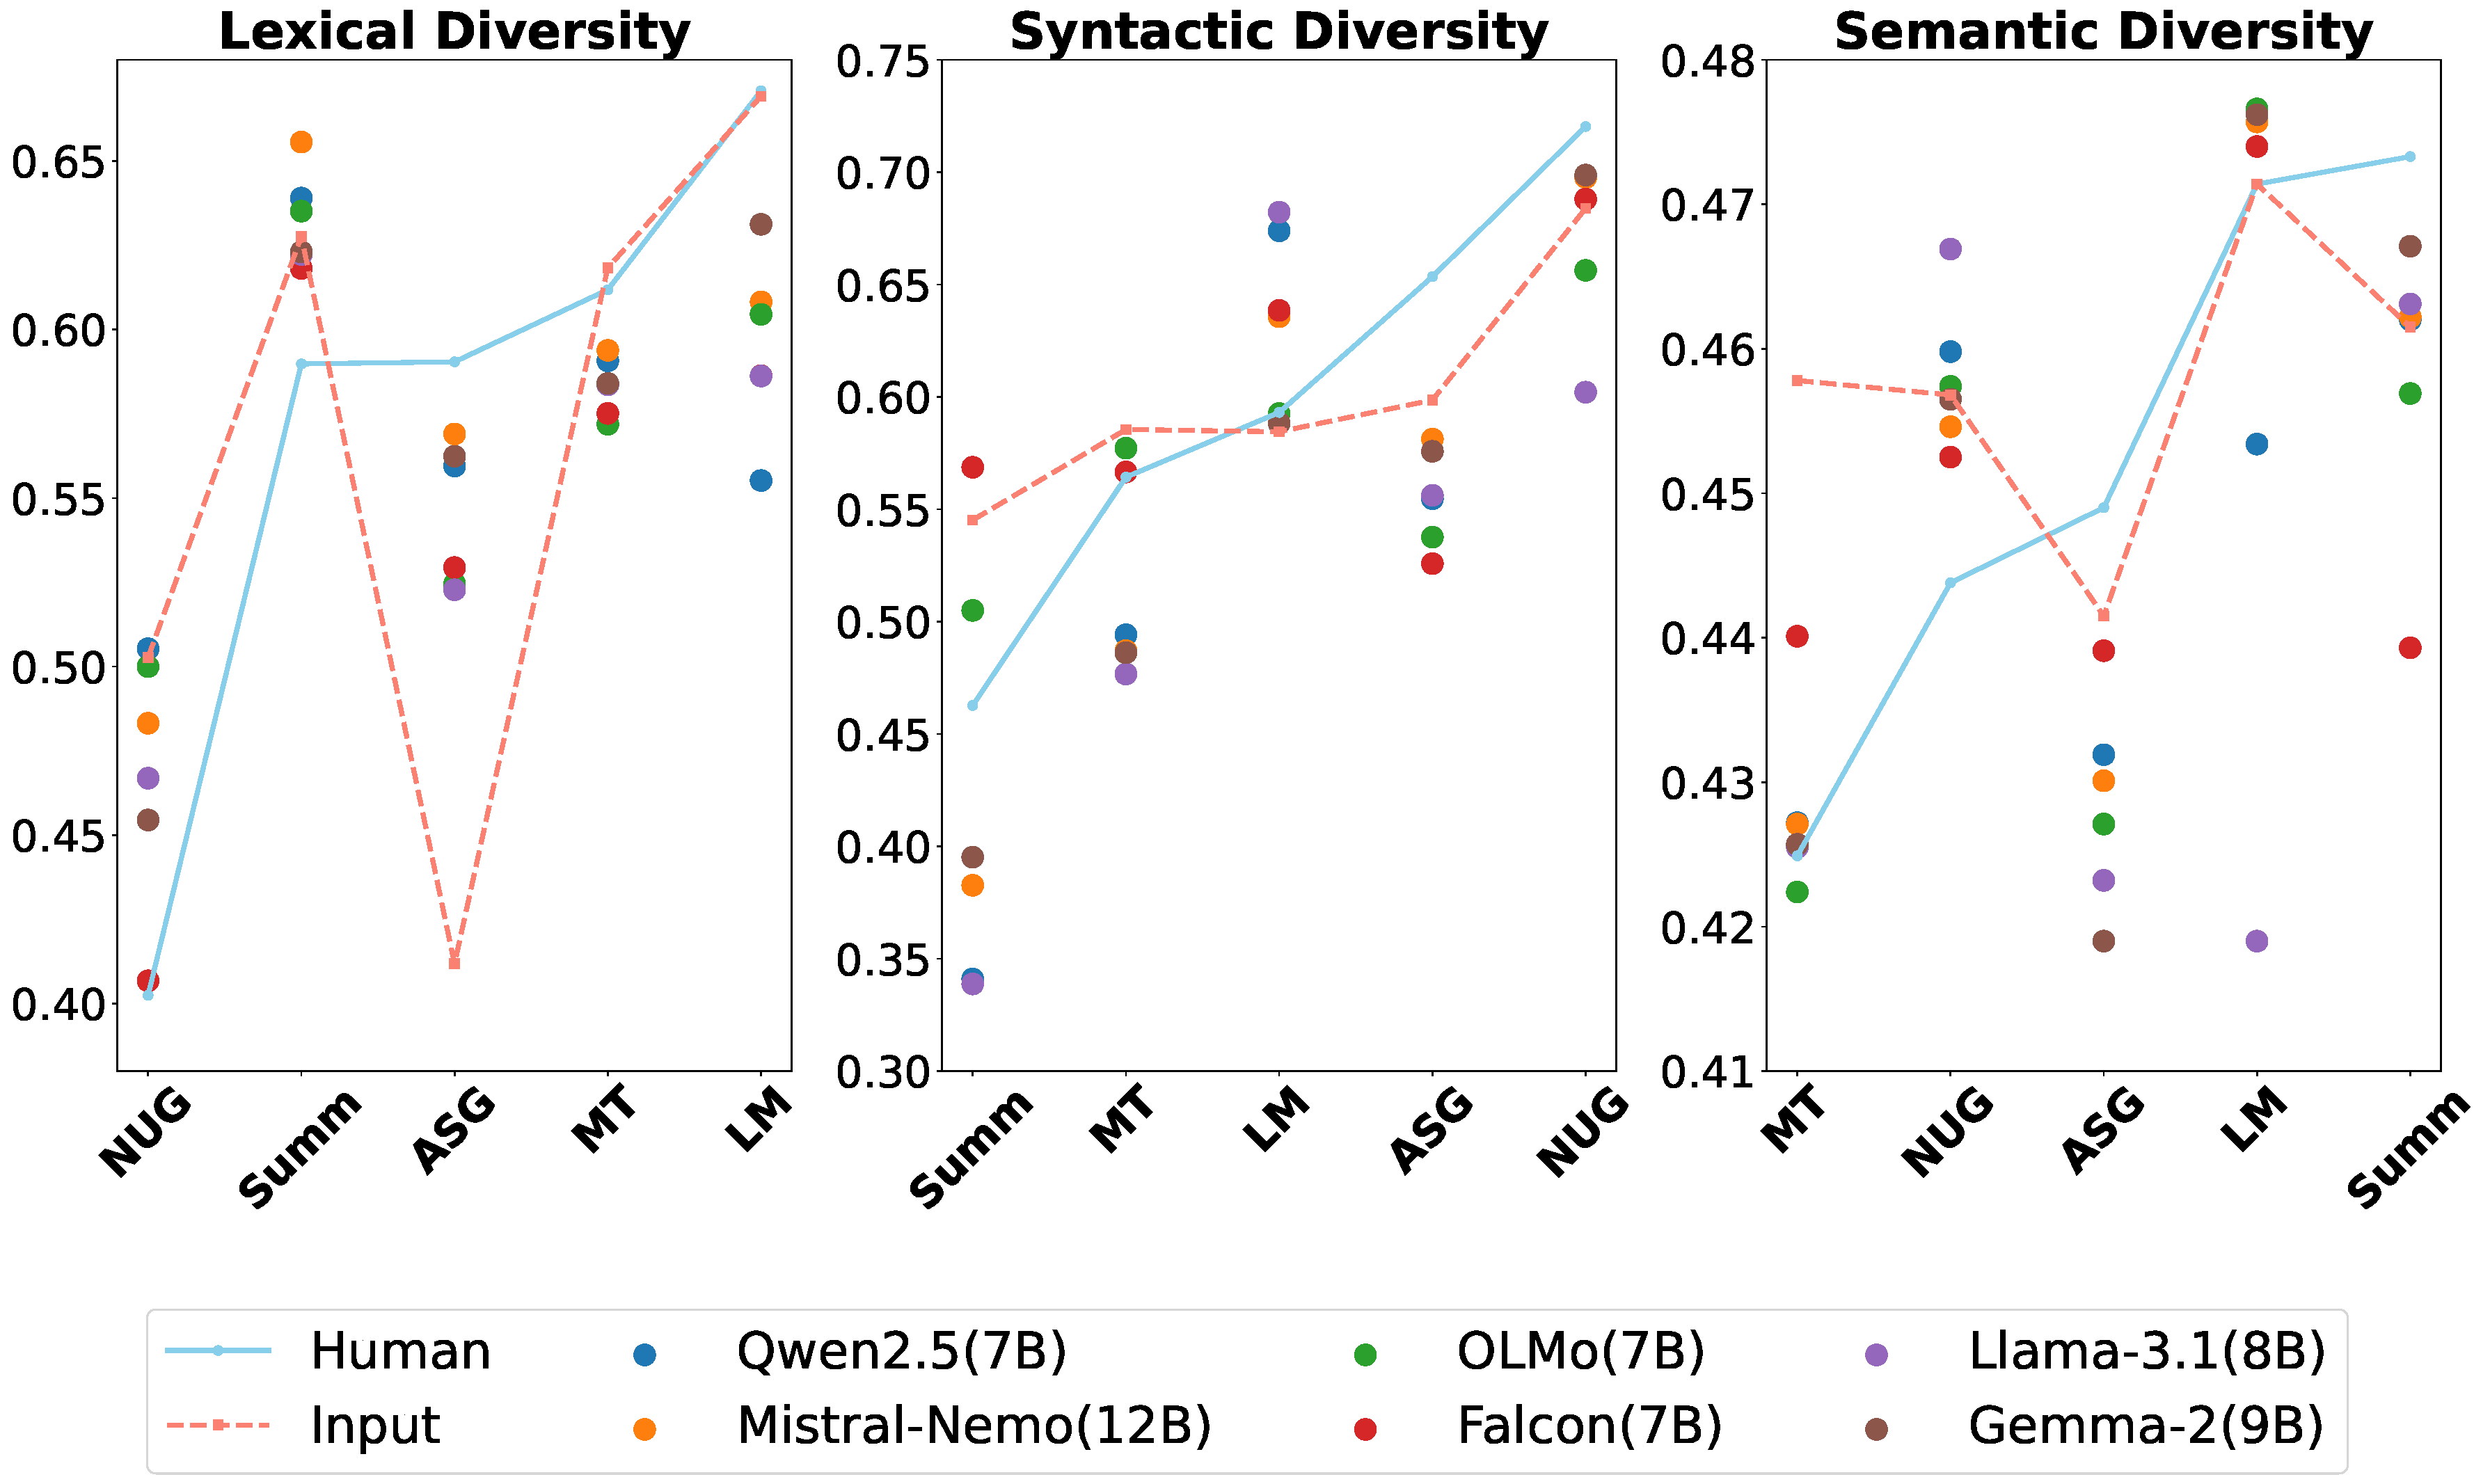
\includegraphics[scale=0.22]{figures/benchmark.pdf}
    \caption{Lingustic diversity benchmarking results for NLG tasks detailed in Table \ref{tab:tasks}.}
    \label{fig:benchmark}
\end{figure*}
% Please add the following required packages to your document preamble:
% \usepackage{booktabs}
% \usepackage{graphicx}
\begin{table*}[ht]
\centering
\resizebox{\textwidth}{!}{%
\begin{tabular}{@{}llll@{}}
\toprule
                    & Dataset                         & Input                               & Output                             \\ \midrule
Language Modeling (\textbf{LM})   & Wikitext-2 \citep{merity2017pointer}    & Block of 128 tokens from Wikipedia & Prediction of the next block      \\
Machine Translation (\textbf{MT}) & WMT-14 \citep{bojar-etal-2014-findings} & News story sentence in French      & Corresponding English translation \\
Summarization (\textbf{Summ})       & XLSUM \citep{hasan-etal-2021-xl}        & Full news article from the BBC     & Summary of the news article     \\
Next Utterance Generation (\textbf{NUG})  & DailyDialog \citep{li-etal-2017-dailydialog}       & Scripted dialogue on general topics & Next utterance of the dialogue       \\
Automatic Story Generation (\textbf{ASG}) & WritingPrompts  \citep{fan-etal-2018-hierarchical} & Story prompt shared by Reddit users & Story continuation based on the prompt \\ \bottomrule
\end{tabular}%
}
\caption{Summary of datasets, inputs, and outputs for benchmarked NLG tasks.}
\label{tab:tasks}
\end{table*}


\subsubsection{Syntactic Diversity}
\label{sec:syn}
Syntactic diversity refers to the range and variety of sentence structures used in a text or set of texts. It assesses how flexibly and creatively different grammatical structures, such as phrases, clauses, and sentence types, are employed. High syntactic diversity suggests varied sentence forms, while low syntactic diversity indicates repetitive or simplistic sentence structures.
Syntactic diversity is a crucial but often neglected aspect of language. Exposure to a variety of syntactic structures helps language learners and models develop a richer understanding of language \citep{aggarwal-etal-2022-towards}. Diverse syntactic forms enhance expressiveness and subtlety in text, impacting its style and tone \citep{edwards1998diversity}. While research on syntactic diversity exists, it typically relies on manual annotation, which can be both costly and error-prone \citep{a89efe5d-217a-3260-b2b1-1437ae204234}.

To address this limitation, we employ a graph-based metric for quantifying syntactic diversity \citep{guo-etal-2024-curious}. This metric relies on a neural parser \citep{qi-etal-2020-stanza} to generate dependency trees from sentences, following the universal dependencies framework. These trees are converted into graph representations, where nodes represent words and edges denote dependency relationships. The nodes are labeled by the PoS tag of each word. The Weisfeiler-Lehman (WL) graph kernel \citep{10.5555/1953048.2078187, JMLR:v21:18-370} is then applied to map these graphs into a vector space. This kernel, based on the WL isomorphism test, positions structurally similar graphs closer together in the vector space. Syntactic diversity is then measured using the average pairwise distance between graphs, formalized as: $\text{Div}_{\text{syn}}(S) = \frac{1}{\binom{n}{2}} \sum_{1 \leq i < j \leq n}WL(s_i, s_j)$. Alternatively, the pairwise distances between the dependency trees could also be measured by the tree editing distance \citep{zhang1989simple}. However, the algorithm to compute the tree editing distance has much higher computational complexity and is thus not scalable to a large set of texts.






\subsubsection{Semantic Diversity}
Semantic diversity refers to the range and variety of meanings or ideas conveyed within a text or set of texts. It evaluates how broadly and uniquely different concepts, topics, or ideas are expressed, reflecting the depth and scope of the content. High semantic diversity suggests a text covers diverse ideas or meanings, while low semantic diversity implies repetition or a narrow focus on specific concepts.
Recent studies \citep{tevet-berant-2021-evaluating, stasaski-hearst-2022-semantic} have pointed out that traditional lexical metrics may not fully capture semantic diversity. Similar words can convey different meanings, and different words can convey similar meanings \citep{pmlr-v80-yarats18a}. 

To address this, we first convert sentences into semantically meaningful embeddings using Sentence-BERT \cite{reimers-gurevych-2019-sentence}. Semantic diversity is then quantified as the dispersion of these embeddings in the semantic space, measured by the average pairwise cosine distance (scaled to the range $[0,1]$) between all embedding vectors: $\text{Div}_{\text{sem}}(S) = \frac{1}{\binom{n}{2}} \sum_{1 \leq i < j \leq n}  \frac{1 + d_{\text{cos}}}{2}(e(s_i), e(s_j))$, where $e$ represents Sentence-BERT embeddings.
%(\texttt{Div\_sem})




\section{Settings for Diversity Benchmarking}
We outline the tasks, datasets, and models used to establish our linguistic diversity benchmark.

\smallskip

\noindent\textbf{Generation tasks}.
To effectively compare the linguistic diversity of LLM outputs across various scenarios, we selected five tasks with progressively increasing levels of ``creativity'': language modeling, machine translation, summarization, automatic story generation, and next utterance generation. Table~\ref{tab:tasks} outlines the inputs, outputs, and datasets associated with each task. Note that the input is combined with a task-specific instruction (e.g., ``Continue the following story:'' for story generation) to construct the final prompt.

% \smallskip

% \noindent\textbf{Language modeling} involves predicting the next word in a sequence based on preceding words and is fundamental to many NLG applications.
% In this paper, we utilize the Wikitext-2 dataset \citep{merity2017pointer} for language modeling. Derived from Wikipedia articles, Wikitext-2 offers a rich and diverse corpus with around 2 million tokens across various topics. We chunk texts into blocks of 128 tokens and ask models to predict the next 128 tokens.
% This diversity makes it an ideal benchmark for evaluating language models. Given that language modeling is integral to the pretraining phase of base LLMs, we assess this task using these base models. For the remaining tasks, we use instruction-tuned LLMs in our experiments.

% \smallskip

% \noindent\textbf{Machine translation} aims to translate text from one language to another while maintaining the original meaning and context. We use the WMT-14 dataset, as detailed in \cite{bojar-etal-2014-findings}, for evaluating translation abilities. WMT-14 is a well-established benchmark containing parallel corpora for multiple language pairs. For our experiments, we focus on a subset of this benchmark that includes French-to-English translations.

% \smallskip

% \noindent\textbf{Summarization} involves creating concise and coherent summaries of longer texts, capturing the essential points while avoiding redundancy. We use the XLSUM dataset \citep{hasan-etal-2021-xl} for this task. XLSUM is a  multilingual summarization dataset featuring news articles in various languages along with their summaries. It is designed to evaluate summarization models across different languages and topics. Our experiments utilize the English subset of the XLSUM dataset.

% \smallskip

% \noindent\textbf{Story generation} centers on producing engaging and coherent narratives from prompts or initial inputs. For this task, we employ the WritingPrompts dataset \citep{fan-etal-2018-hierarchical}, which comprises prompts and corresponding stories contributed by Reddit users. The dataset includes a wide variety of prompts, encouraging diverse and creative responses, making it a valuable resource for evaluating models in generating human-like stories.

% \smallskip

% \noindent\textbf{Dialogue generation} involves crafting natural and contextually appropriate responses in conversations on any topic. We use the DailyDialog dataset \citep{sai-etal-2020-improving} for testing the linguistic diversity of LLM responses in a multi-turn conversation. DailyDialogue++ is an extended version of the DailyDialogue \citep{li-etal-2017-dailydialog} dataset and includes conversations from various everyday scenarios.

For each task, we randomly select 10K samples from the original dataset. To obtain the benchmark results, we decode the outputs for all models and tasks using a combination of nucleus sampling (t=0.6) and top-k sampling (k=0.9). We further analyze in Section \ref{sec:decoding} the impact of different decoding parameters on output diversity.




\begin{figure*}[ht]
\begin{minipage}{0.55\linewidth}\centering
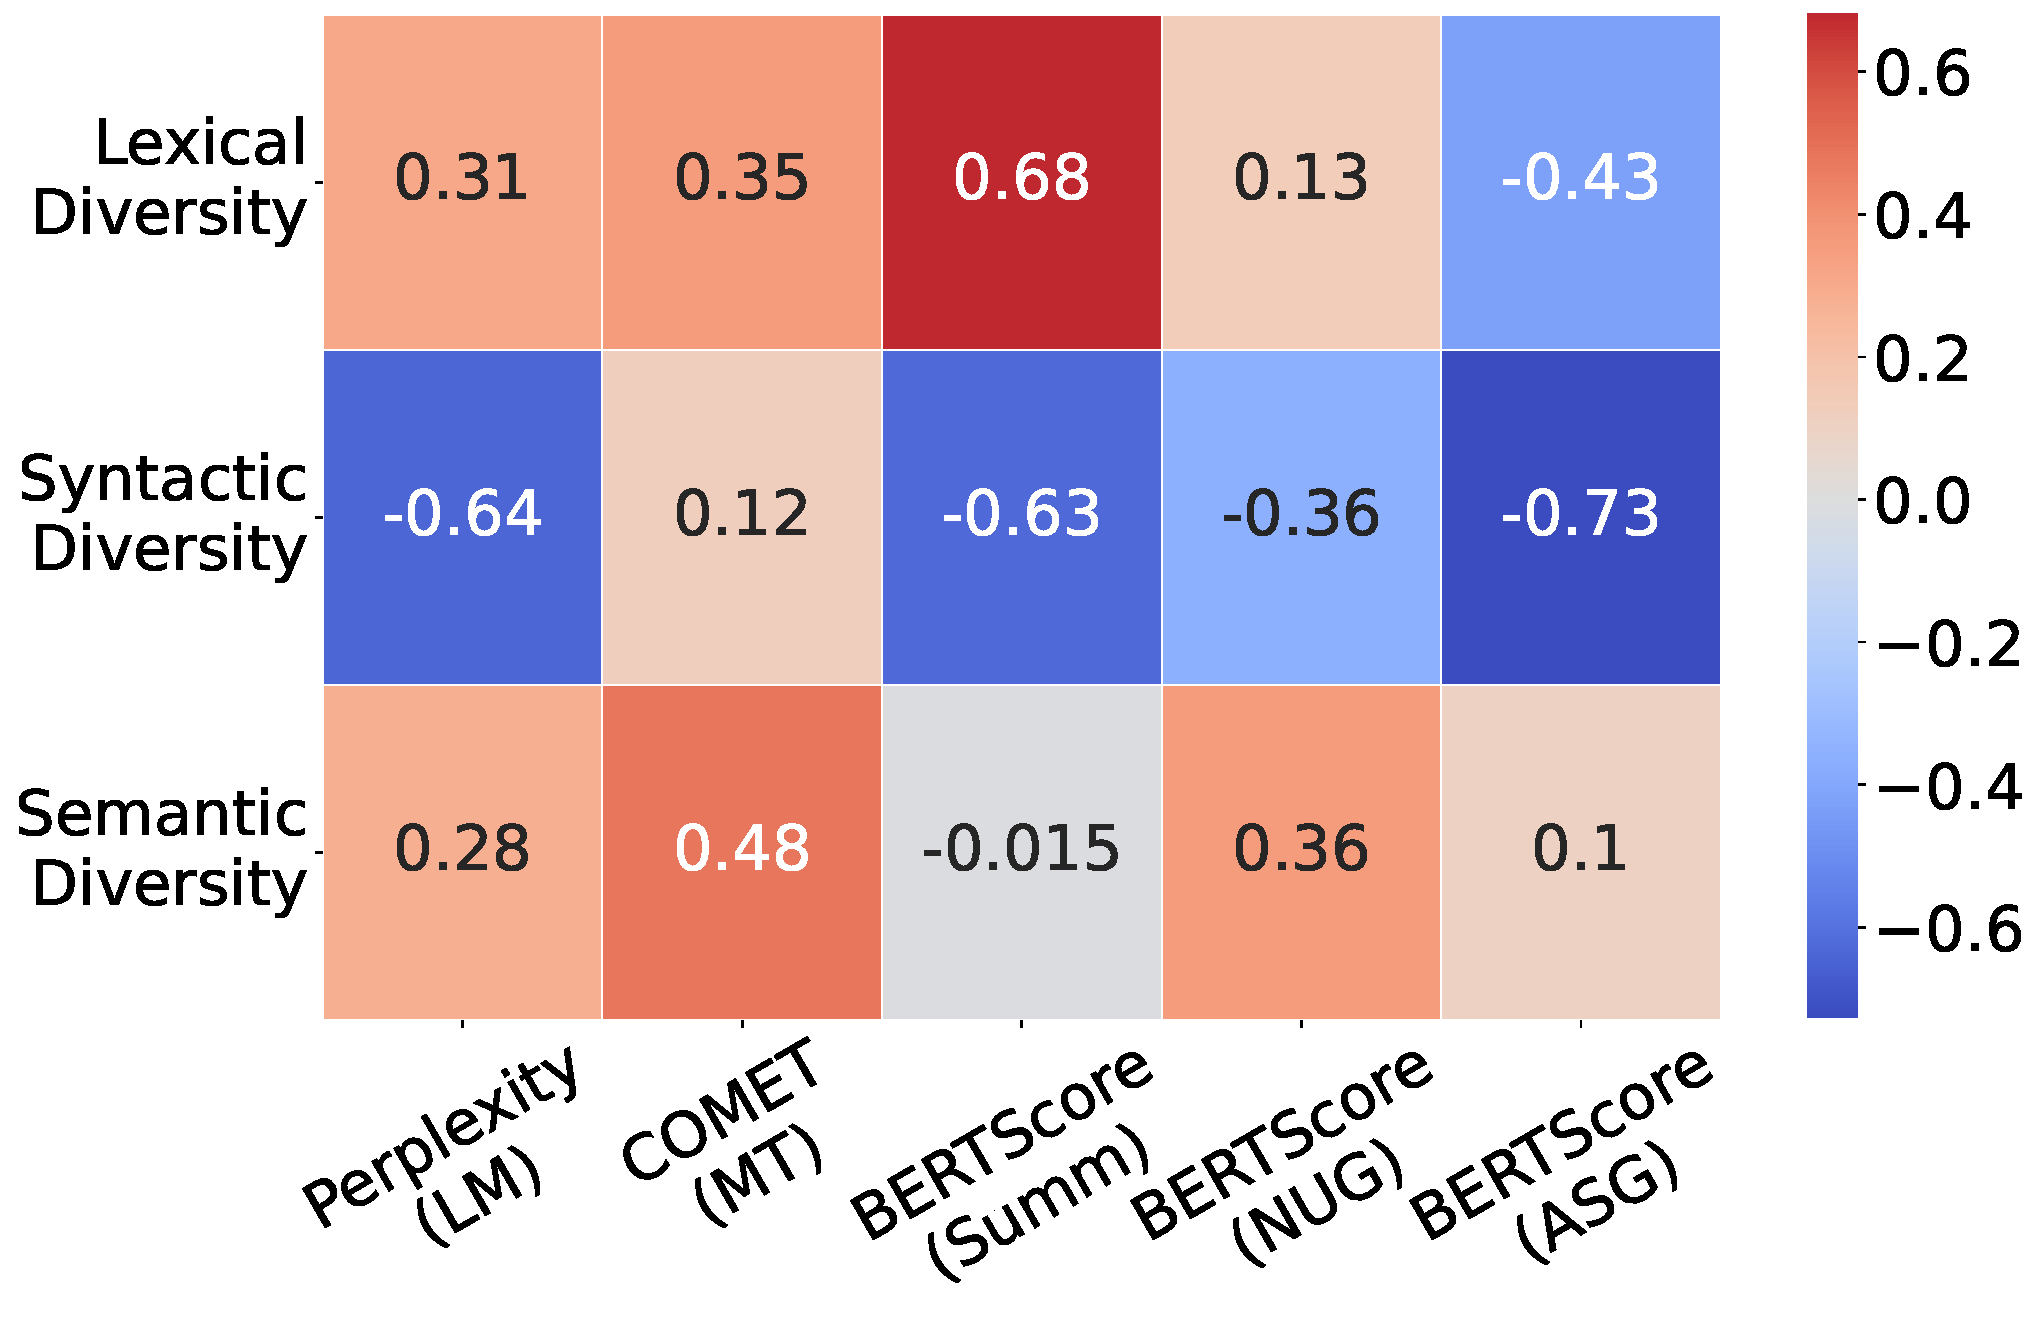
\includegraphics[height=9.3\baselineskip]{figures/correlation_qual_div.pdf}
\caption{Pearson correlation matrix between diversity metrics and quality metrics.}
%The abbreviations of task names are the same as in Figure~\ref{fig:benchmark}.
%The correlation is computed individually for each of the 5 tasks because different tasks have different quality metrics
\label{fig:correlation_qual_div}
\end{minipage}\hfill
\begin{minipage}{0.4\linewidth}\centering
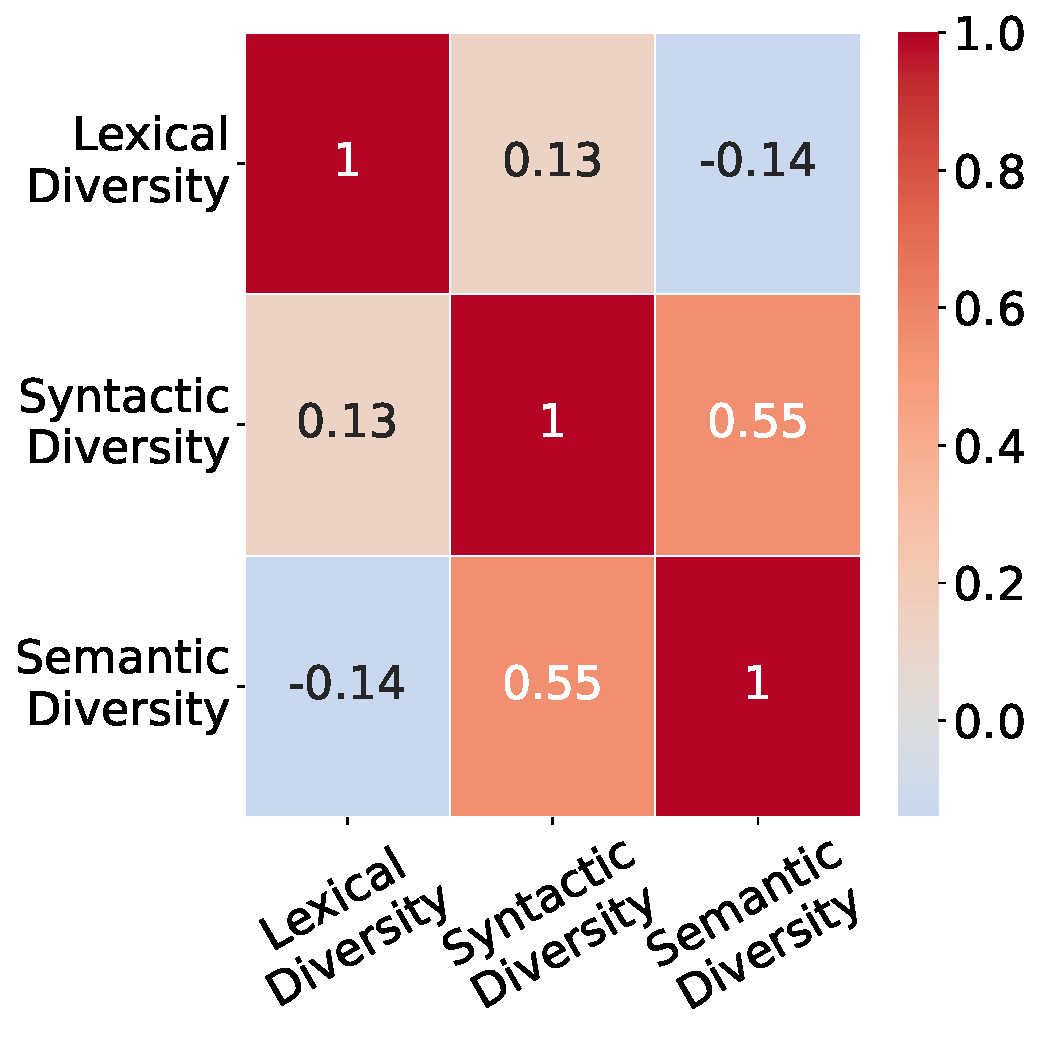
\includegraphics[height=9.3\baselineskip]{figures/correlation_div.pdf}
\caption{Pearson correlation matrix between different diversity metrics.}
%The correlation is computed across all 5 tasks.
\label{fig:correlation_div}
\end{minipage}
\end{figure*}

\smallskip


\noindent\textbf{Large language models}.
We evaluate the following families of models: Llama \citep{dubey2024llama}, Mistral \citep{jiang2023mistral}, Olmo \citep{groeneveld2024olmo}, Gemma \citep{team2024gemma}, Qwen \citep{yang2024qwen2}, Falcon \citep{almazrouei2023falcon}.
%The comparison of these models across various key characteristics is provided in Appendix \ref{app1}, including multilinguality, alignment, and the inclusion of synthetic data in training.
To ensure comparability, we select the latest version of each model family that is closest in scale to 7 billion parameters. The scale selected for each model is specified in the legend of Table~\ref{fig:benchmark}. We purposefully include models developed by organizations from different countries to be culturally inclusive. For language modeling, we use base models. For all other tasks, we employ instruction-tuned versions. %When using models with a system input field in their instruction template, we place the task instruction prompt in the system input and the sample-specific information in the user input. For models without a system input field, we prepend the task instruction to the user input.






    



% \begin{figure*}[h!]
%     \centering
%     \begin{subfigure}[b]{0.35\textwidth}
%         \centering
%         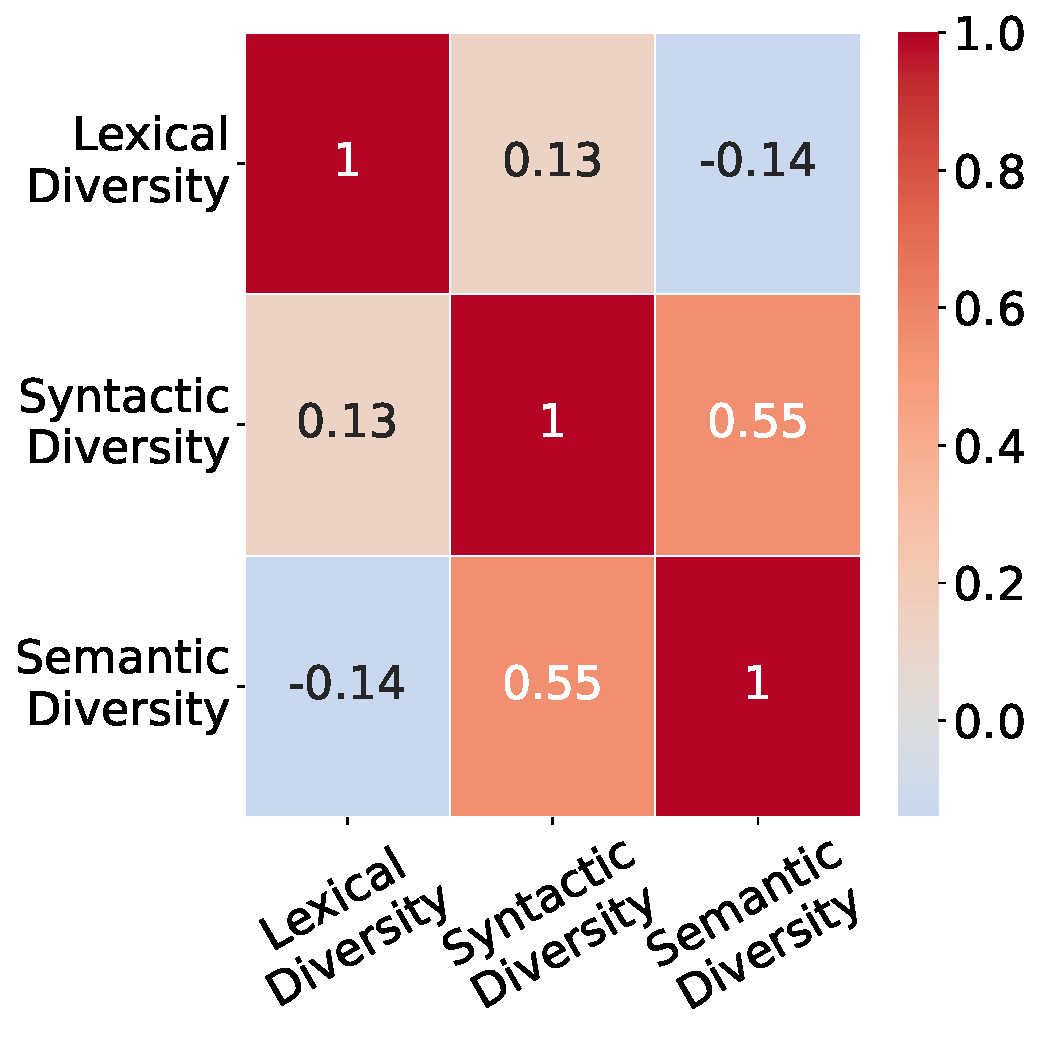
\includegraphics[width=\textwidth]{figures/correlation_div.pdf}
%         \caption{Pearson correlation matrix between different diversity metrics. The correlation is computed across all 5 tasks.}
%         \label{fig:correlation_div}
%     \end{subfigure}
%     \hfill
%     \begin{subfigure}[b]{0.57\textwidth}
%         \centering
%         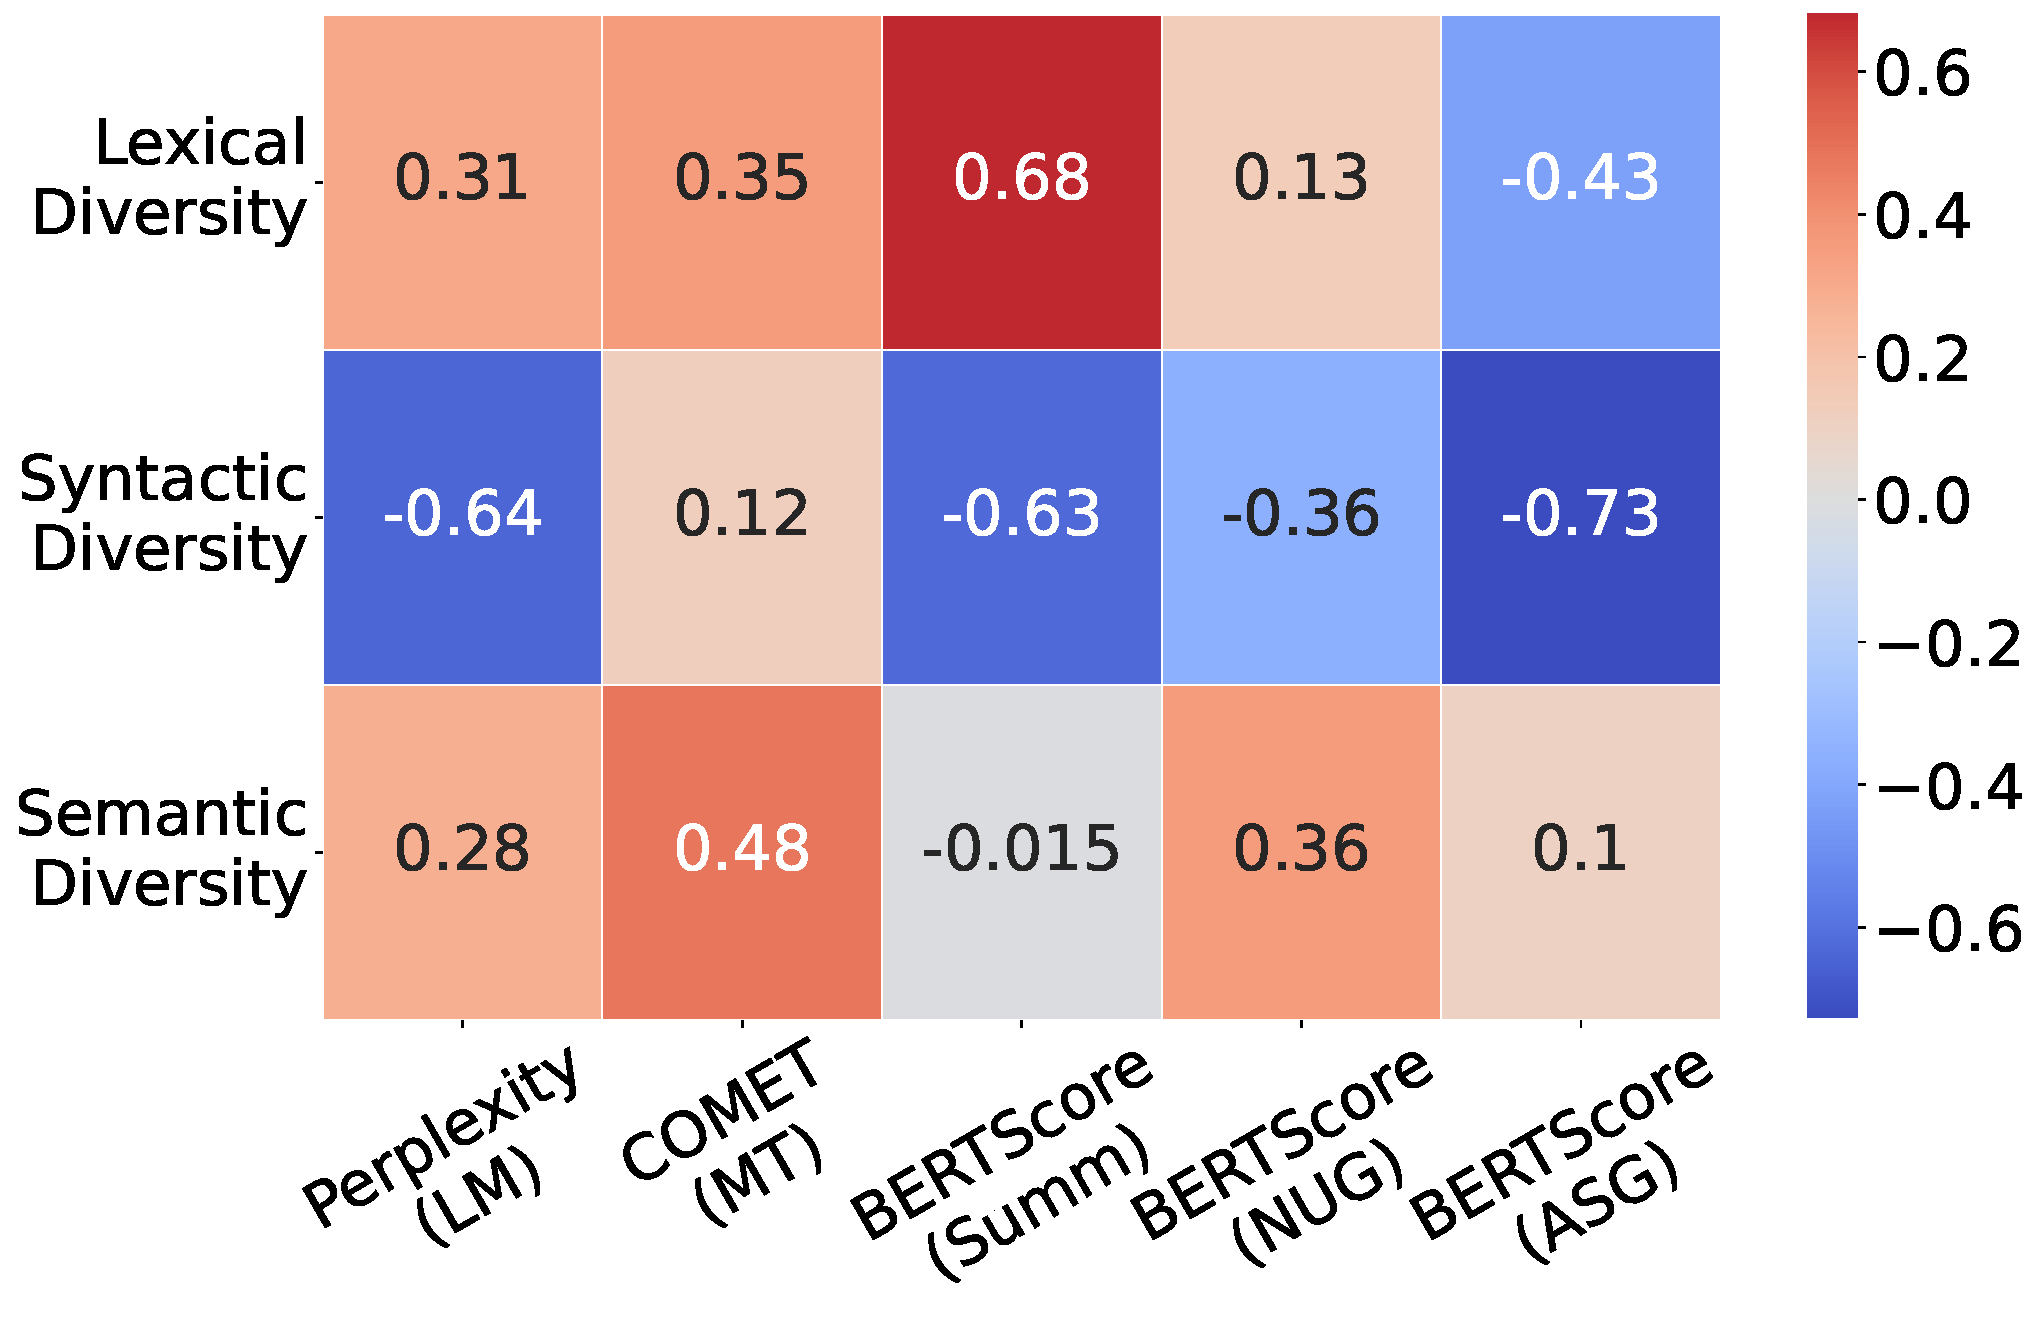
\includegraphics[width=\textwidth]{figures/correlation_qual_div.pdf}
%         \caption{Pearson correlation matrix between diversity metrics and quality metrics. The correlation is computed individually for each of the 5 tasks because each task has a different quality metric.}
%         \label{fig:correlation_qual_div}
%     \end{subfigure}
%     \hfill
    
%     \caption{Correlation analysis of diversity and quality metrics.}
%     \label{fig:results}\end{figure*}

\section{Results for Diversity Benchmarking}\label{sec:benchmarking_results}

Figure~\ref{fig:benchmark} presents the benchmarking results of linguistic diversity across various tasks. Round dots represent the diversity of model outputs, while solid lines represent human reference outputs. Dashed lines depict the diversity of task-specific inputs (as detailed in Table~\ref{tab:tasks}), reflecting the conditions under which the outputs were generated. Tasks are organized in ascending order of human reference diversity for each aspect of diversity. For the machine translation task, the inputs are in French; hence, semantic diversity is measured using a multilingual SentenceBERT~\citep{reimers-gurevych-2020-making}, and syntactic diversity is evaluated with a French-specific dependency parser. As a result, these scores may not be directly comparable to those for English. We analyze the results in Figure \ref{fig:benchmark} in Sections \ref{sec:ComparisonTasksModels} and \ref{sec:ComparisonHumansModels}. 
%For translation and summarization, the content of the output generations are highly dependent on the prompts, thus their linguistic diversity scores should also be correlated. 
%The diversity of human reference outputs serves as a baseline for interpreting whether the model under or over represents the diversity for each task.

In this section, we first analyze metric correlations in Section \ref{sec:CorrelationStudy}, then compare diversity scores across tasks and models in Section \ref{sec:ComparisonTasksModels}.	Finally, we perform a case study on syntactic diversity in story generation, comparing human and model outputs in Section \ref{sec:ComparisonHumansModels}.

\subsection{Correlation Study}\label{sec:CorrelationStudy}

%We first study the correlation between diversity and quality metrics, and then move on to study the correlation between diversity metrics for different aspects.

\smallskip
\noindent\textbf{Correlation between diversity and quality}.
%The interpretation of linguistic diversity scores is meaningful only when the quality of the generated outputs meets a certain threshold. 
%For example, a random combination of nonsensical tokens might display high lexical diversity but still constitute undesirable output. 
As noted in Section \ref{subsec:human}, diversity matters only if the text is of plausible quality.
Figure~\ref{fig:correlation_qual_div} illustrates the correlation between diversity and quality in model outputs, using task-specific automatic metrics as quality indicators. For the language modeling task, perplexity is used to evaluate the model's performance on reference text continuations. For machine translation, we use COMET~\citep{rei-etal-2020-comet}, which takes into account both the source text and reference translation. For the remaining three tasks, BERTScore~\citep{bert-score} is used to measure the relevance between inputs and outputs. However, for these last three tasks with a subjective nature, this relevance score serves only as a proxy for quality, as automatic metrics for such tasks generally exhibit low correlation with human judgments~\citep{10.1162/tacl_a_00689, liu-etal-2023-g}.

%Given the subjective nature of these three tasks, relevance to the input is only one quality aspect that is the easiest to measure. To ensure the overall quality of model outputs on these tasks, we also use GPT-4 as a judge~\citep{zheng2023judging}. In summarization, we ask GPT-4 to evaluate based on the criteria of coherence, consistency, relevance, and fluency~\citep{liu-etal-2023-g}. For story generation, the criteria are relevance, coherence, empathy, surprise, engagement, and complexity~\citep{10.1162/tacl_a_00689}. For dialogue generation, the criteria are helpfulness, relevance, accuracy, depth, creativity, and level of detail~\citep{zheng2023judging}. The GPT-4 evaluations indicate that all models achieve high levels of performance, often comparable to human outputs. However, we exclude GPT-4 scores from the correlation analysis due to their narrow range (typically concentrated between 7 and 9 on a 10-point scale).

%We compute the Pearson correlations between diversity metrics and the previously described quality metrics. Given a model $m$ and task $t$, its quality score is noted as $Qual(G_m(P_t))$, and an aspect of diversity score is noted as $Div(G_m(P_t))$. For each task $t$, we calculate the correlation between the lists $[Qual(G_m(P_t))]_{m \in \{\text{all models}\}}$ and $[Div(G_m(P_t))]_{m \in \{\text{all models}\}}$ to determine the correlation between quality and each diversity aspect. 

Our results show a positive correlation between quality and lexical as well as semantic diversity in model outputs.	 %suggesting that higher diversity in these aspects tends to correspond with better scores from automatic quality metrics. 
In contrast, syntactic diversity often exhibits negative correlations, where higher syntactic diversity is associated with lower quality scores.
This may be attributed to the tested domains inherently exhibiting low ground-truth syntactic diversity (e.g., in language modeling) or to the limitations of quality metrics in recognizing the value of syntactic variation (e.g., in summarization, automatic story generation, and next utterance generation).
\textit{These findings highlight the need to report diversity metrics alongside quality metrics for comprehensive evaluation.}

\smallskip
\noindent\textbf{Correlation between diversity aspects}.\label{sec:correlation}
The correlations between different diversity aspects are shown in Figure \ref{fig:correlation_div}, revealing a moderate positive correlation between syntactic and semantic diversity (0.55).
%suggesting that syntactic variation can enhance semantic richness to some extent. 
However, lexical diversity shows a weak positive relationship with syntactic diversity (0.13) and a slight negative correlation with semantic diversity (-0.14), indicating that \textit{the richness of vocabulary is independent from the variety of grammatical structures and meaning}.


% Please add the following required packages to your document preamble:
% \usepackage{booktabs}
% \usepackage{graphicx}
\begin{table*}[ht]
\centering
\resizebox{\textwidth}{!}{%
\begin{tabular}{@{}lllll@{}}
\toprule
             & \multicolumn{2}{c}{\textbf{Human}}         & \multicolumn{2}{c}{\textbf{Language Models}}           \\
             & \textbf{POS tag n-gram} & \textbf{Example} & \textbf{POS tag n-gram} & \textbf{Example} \\ \midrule
\textbf{n=3} & (ADV, ADV, ADP)         & right along with & (PRON, NOUN, ADJ)       & her voice soft   \\
\textbf{n=4} & (VERB, ADP, DET, NOUN)          & picking up the pieces         & (NOUN, CCONJ, NOUN, PRON)           & carvings and symbols that          \\
\textbf{n=5} & (DET, NOUN, ADP, DET, NOUN)     & the cackling of the fire      & (PRON, NOUN, VERB, ADP, NOUN)       & its feathers stained with blood    \\
\textbf{n=6} & DET, ADJ, NOUN, ADP, DET, NOUN) & the old woman down the street & (ADJ, NOUN, ADP, NOUN, CCONJ, NOUN) & particular focus on time and space \\ \bottomrule
\end{tabular}%
}
\caption{Examples of syntactic patterns favored by either humans or models are illustrated using n-grams of POS tags. Human patterns are derived from human dependency trees that are not within the model dependency tree neighborhoods, while model patterns have high frequency in model dependency trees and low frequency in human dependency trees.}
\label{tab:examples}
\end{table*}

% Please add the following required packages to your document preamble:
% \usepackage{booktabs}
% \usepackage{graphicx}
\begin{table}[ht]
\centering
\resizebox{\columnwidth}{!}{%
\begin{tabular}{@{}lllllll@{}}
\toprule
                   & \textbf{Llama} & \textbf{Mistral} & \textbf{Qwen} & \textbf{Gemma} & \textbf{Falcon} & \textbf{OLMo} \\ \midrule
\textbf{Precision} & 99.20                 & 99.20                     & 99.47               & 99.07               & 99.63              & 99.73            \\
\textbf{Recall}    & 35.20                 & 65.87                     & 75.27               & 37.97               & 75.00              & 39.40            \\ \bottomrule
\end{tabular}%
}
\caption{Comparison of dependency tree distributions between humans and models.}
\label{tab:precision_recall}
\end{table}


%\smallskip


\subsection{Comparison Across Tasks and Models} \label{sec:ComparisonTasksModels}

We now examine the results in Figure \ref{fig:benchmark} to assess human diversity results across tasks, compare model diversity against human diversity, and finally evaluate the diversity performance across different models.

\smallskip
\noindent\textbf{Human output diversity}.
\textit{Human-level diversity varies across tasks, with no clear correlation observed among different aspects.}
Notably, utterances in human dialogue exhibit the lowest lexical diversity and the highest syntactic diversity, unlike the written text present in the remaining four categories.	
%These findings align with established linguistic research on conversations:
%Speakers tend to repeat lexical materials from previous discourse, either their own or their interlocutor's \citep{levelt1982surface, dubuisson-duplessis-etal-2017-automatic};
The low lexical diversity may be attributed to the conversations being specifically scripted for English learners to practice daily-life dialog. These dialogs focus on generic topics, leading to a limited range of vocabulary. In contrast, the high syntactic diversity can be explained by the inherent spontaneity of conversational language, where different speakers tend to vary significantly in their use of syntactic structures \citep{healey2014divergence, dubuisson-duplessis-etal-2017-automatic}.

\smallskip
%analyze creativity levels of different tasks and their expected diversity
%We believe that some of the excess diversity might be due to undesired noisy generations.
%except in the syntactic diversity for summarization and translation
\noindent\textbf{Model output diversity}.
\textit{LLMs generally lack diversity compared to humans, especially remarkable for tasks demanding high levels of creativity, such as story generation.}
Overall, the scores of different LLMs across tasks and diversity aspects tend to resemble each other due to the use of similar development procedures, architectures, and datasets.
Compared to human outputs, LLMs generally exhibit less diversity by a considerable margin, with only a few exceptions. This is especially evident in the task of story generation, which demands the highest levels of creativity and freedom of expression, LLMs consistently lag behind humans in all three diversity aspects. In contrast, for tasks like next utterance generation, LLMs surpass human references in both lexical and semantic diversity. This discrepancy arises because the DailyDialog dataset focus on generic, everyday topics designed for English language learning, while LLMs, unconstrained by this context, frequently steer conversations toward more complex topics.




\smallskip
\noindent\textbf{LLM comparisons}.
% if the model is trained on more tokens does it improve the lexical diversity? (token count is the best available proxy of the initial lexical diversity of the pretraining corpus)
While the overall performance of the models appears to be similar, in-depth comparisons showcase notable differences.		
\textit{Models pretrained on fewer tokens, such as Falcon and OLMo, consistently generate outputs with lower lexical diversity.} Specifically, Falcon and OLMo are pretrained on 1.5T and 2.7T tokens, respectively, compared to Llama-3.1, which is trained on 15T tokens.
However, this effect is not observed for syntactic or semantic diversity.
\textit{Models with less strict data filtration exhibit greater diversity in creative tasks}, such as story generation.	
For example, Qwen2.5, which filters data exclusively for quality, exhibits significantly higher diversity in story generation across all aspects compared to Llama-3.1, Gemma-2, and OLMo, whose data is extensively filtered for quality, privacy, and safety.


\begin{figure*}[ht]
    \centering
    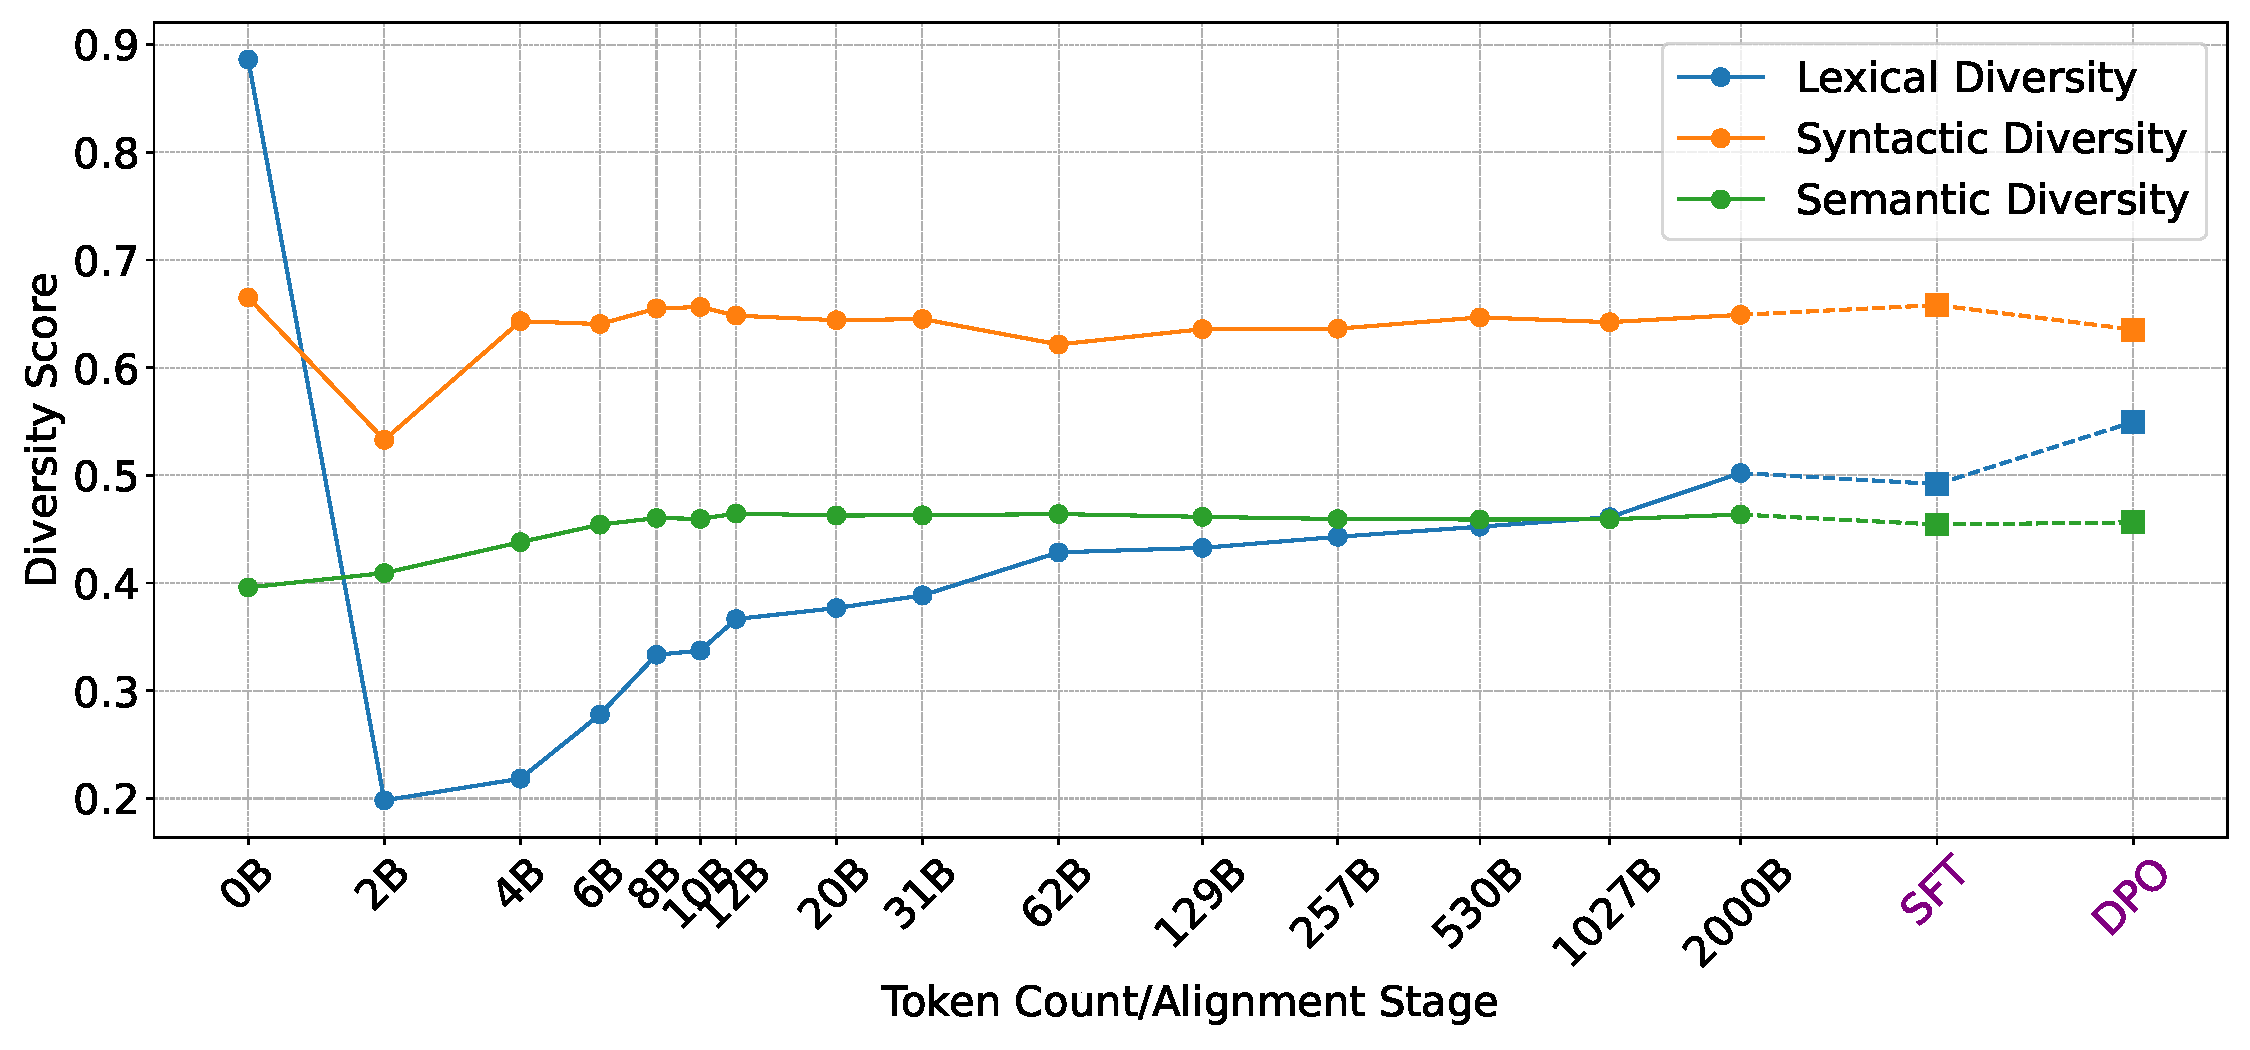
\includegraphics[width=0.85\textwidth]{figures/olmo_diversity_plot.pdf}
    \caption{Linguistic diversity metrics after different LLM training stages. The pretraining stage is broken into various steps with increasing token counts, which are presented on a log scale for visualization. Experiments are conducted with the OLMo model on the story generation task.}
    \label{fig:olmo}
\end{figure*}


\begin{figure*}[h]
    \centering
    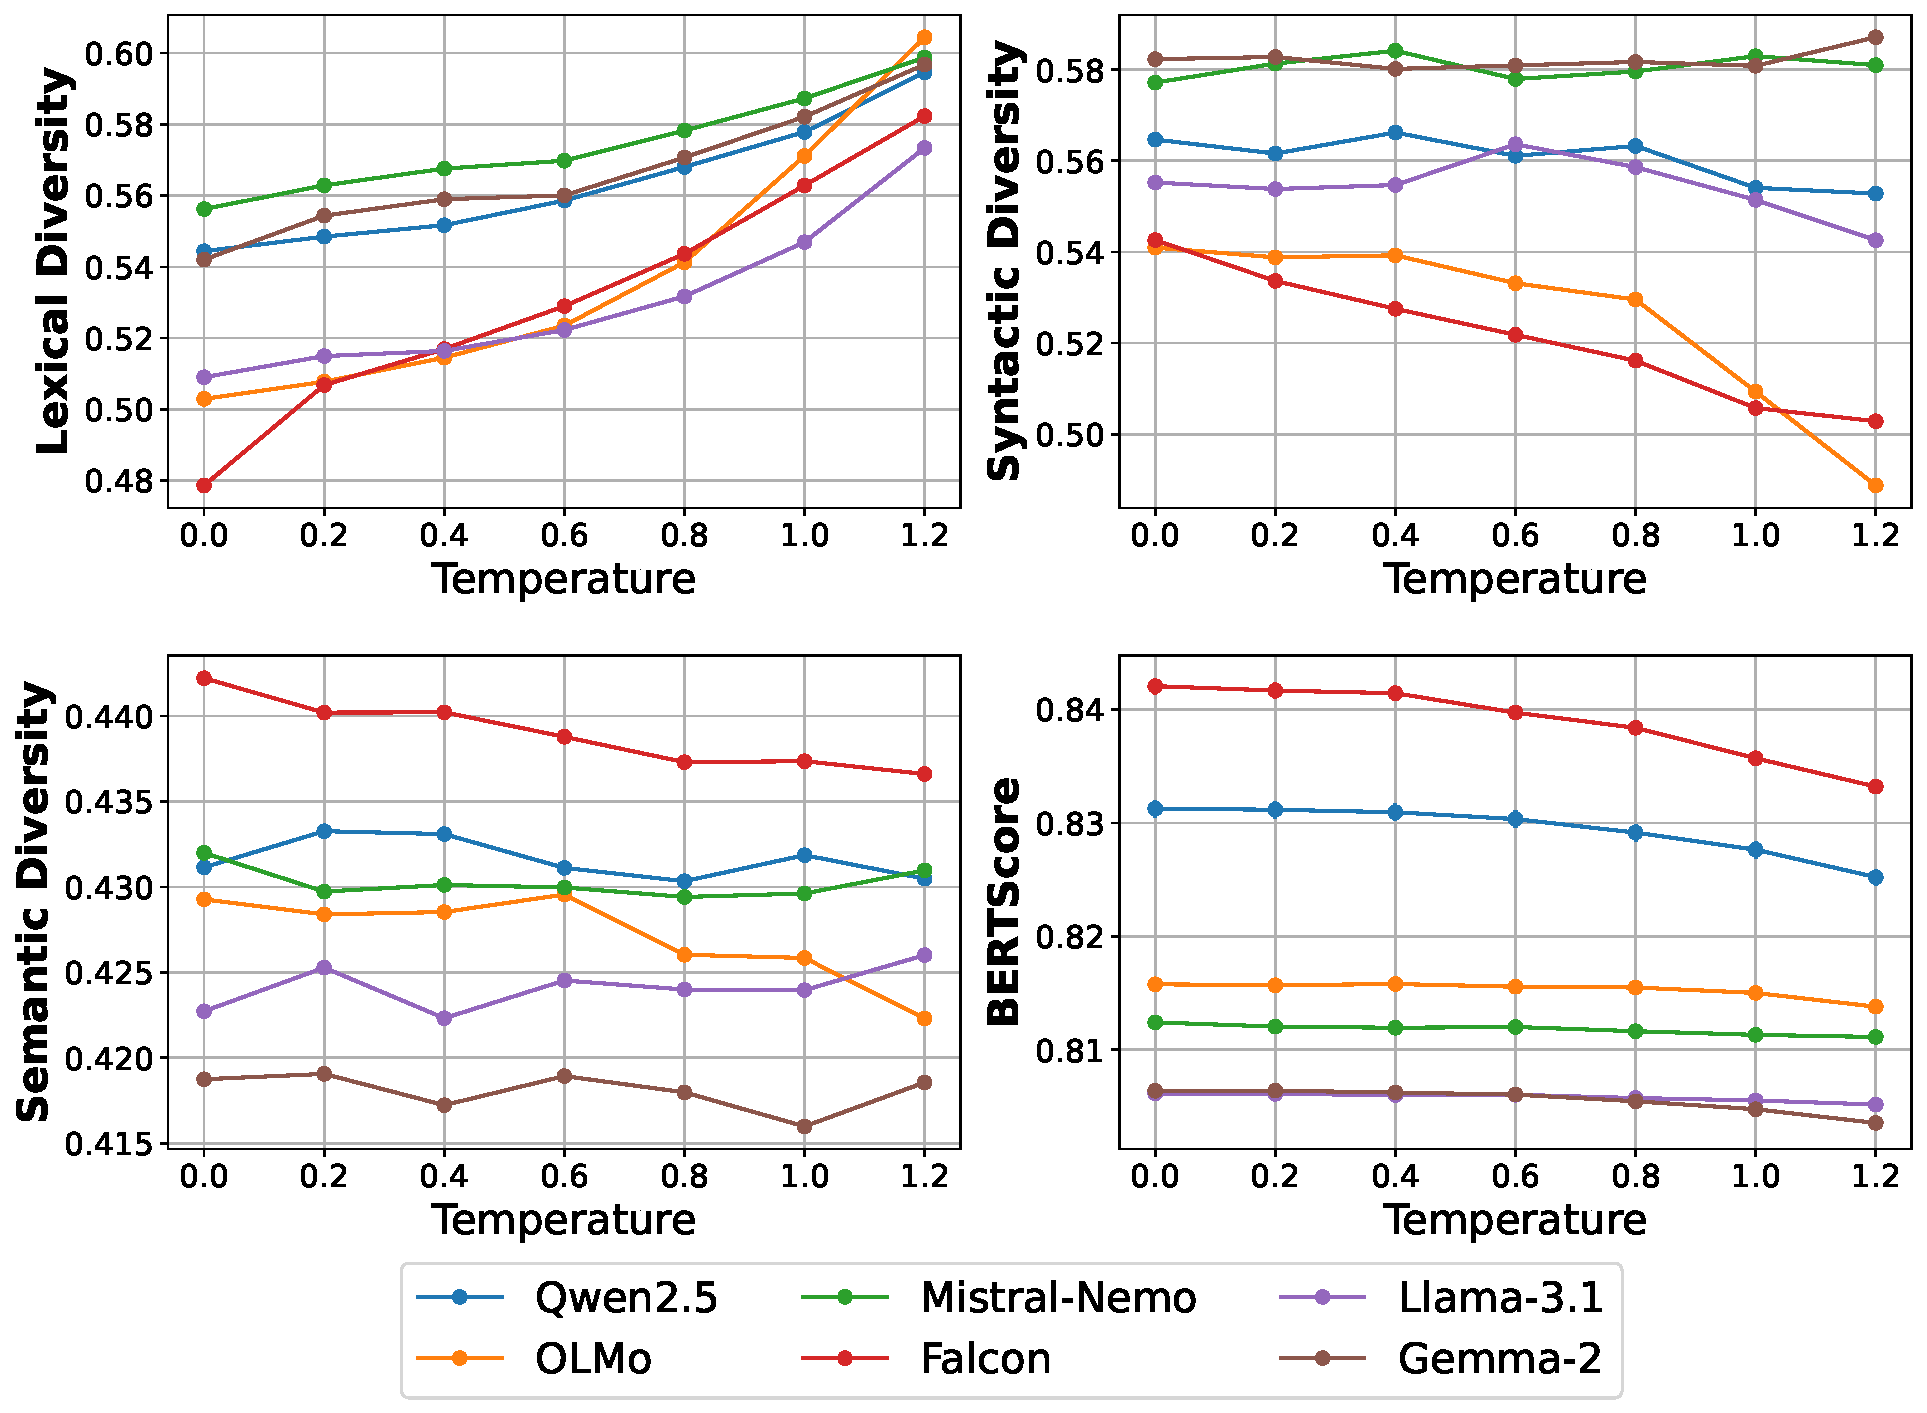
\includegraphics[width=0.91\textwidth]{figures/decoding.pdf}
    \caption{Impact of decoding parameters. Experiments are conducted on the story generation task.}
    \label{fig:decoding}
\end{figure*}



%\noindent\textbf{Inclusion of synthetic data}.

%\noindent\textbf{Multilinguality}.




\subsection{Comparing Syntactic Diversity Between Humans and Models}\label{sec:ComparisonHumansModels}



To further compare humans and models, we conduct a case study on syntactic diversity using dependency tree distribution. Syntactic diversity is chosen as it is less explored than lexical and semantic diversity. Moreover, syntactic patterns reflected by POS tag n-grams are more generalizable than lexicon n-grams and more interpretable than semantic embeddings.


%We make use of the precision-recall framework proposed by \citet{le-bronnec-etal-2024-exploring}. This framework relies on GPT-2 embeddings, followed by PCA and k-means clustering, to estimate the supports of the human and model text distributions. In this approach, the diversity gap (percentages of the human distribution that odel outputs cannot cover) is measured by recall, representing the overlap of the generated distribution with the reference distribution, while precision assesses the quality of the generated texts.

We adopt the Precision-Recall framework proposed by \citet{le-bronnec-etal-2024-exploring}. 
%Recall measures the coverage of the human text distribution by the LLM text distribution, while precision assesses the the coverage of the LLM text distribution by the human text distribution. The distributions are estimated based on GPT-2 embeddings.
In our study, we substitute the original GPT-2 embeddings with the distribution of dependency trees, allowing for a fully interpretable analysis of syntactic structural differences between human and model outputs. 
Precision thus quantifies the percentage of model-generated dependency trees that fall within the neighborhood of human-written ones, while recall measures the percentage of human-written dependency trees within the neighborhood of model-generated ones.
The method for computing the distance matrix between dependency trees is detailed in Section~\ref{sec:syn}. All other hyper-parameters remain consistent with the original work \citep{le-bronnec-etal-2024-exploring}. 

Table~\ref{tab:precision_recall} presents the precision and recall scores for all evaluated models on the story generation task. The results reveal that all models exhibit near-perfect precision, indicating that almost all generated sentences are syntactically plausible. However, the recall scores are significantly lower across all models, highlighting their inability to cover the full diversity of human syntax. \textit{This points to a notable gap between models and humans in syntactic diversity for the story generation task requiring high creativity}.

To further illustrate these findings, Table~\ref{tab:examples} lists examples of syntactic patterns (POS tag n-grams) that are frequently found in human dependency trees but are missing from the model-generated ones. Conversely, we also identify syntactic patterns that models over-generate but are less common in human outputs. Recent studies~\citep{shaib-etal-2024-detection} indicate that models often memorize syntactic templates encountered during pretraining, which are rarely overwritten during fine-tuning. This suggests that the observed gap in syntactic patterns may stem from a mismatch between pretraining and downstream task domains.




\section{Factors Influencing LLM Diversity}

In this section, we explore key factors that may influence the diversity of LLM outputs. The factors under consideration include decoding parameters, pretraining token counts, instruction tuning, model scale, and quantization. For decoding parameters and instruction tuning, we conduct experiments across all models. We employ OLMo for assessing the impact of pretraining token counts, which 
%is a series of Open Language Models specifically designed to advance the science of language models. OLMo 
provides full access to its pretraining datasets, training code, and model weights at various checkpoints throughout its development. Since OLMo models are available in only two sizes, we additionally leverage Qwen2.5 models \citep{yang2024qwen2} to investigate the effects of model scale and quantization.

All experiments in this section are conducted for story generation, selected for its minimal constraints and high emphasis on creativity, making it an ideal benchmark for linguistic diversity. Additionally, as illustrated in Figure~\ref{fig:benchmark}, we observe that all models substantially underperform relative to human scores in terms of diversity metrics on the story generation task.




\subsection{Impact of Training Stages}\label{sec:training_stages}

OLMo was pretrained on the Dolma corpus \citep{soldaini-etal-2024-dolma} before going through supervised fine-tuning (SFT) on Tulu v2 \citep{ivison2023camelschangingclimateenhancing} and direct preference optimization (DPO) \citep{rafailov2023direct} on Ultrafeedback \citep{cui2024ultrafeedback}. DPO is performed on top of the model that underwent SFT. We take different checkpoints throughout the pretraining stage as well as the models after SFT and DPO. We use them to perform the story generation task and analyse the linguistic diversity of outputs. The results are presented in Figure \ref{fig:olmo}.
Initially, lexical diversity is exceptionally high, as expected for an untrained model that generates random tokens. This metric drops sharply after the first checkpoint (2B tokens) but then gradually increases throughout the pretraining process, without reaching saturation. In contrast, syntactic diversity also experiences a sharp decline early on; however, it saturates much more quickly, fluctuating within a narrow range afterward. Semantic diversity shows a steady increase from the beginning but also saturates relatively quickly. \textit{These observations suggest that while increasing training data generally improves lexical diversity, alternative strategies are needed to enhance syntactic and semantic diversity.}

In the later stages, beyond pretraining, SFT has minimal impact on any diversity metric, while DPO leads to a decrease in syntactic diversity and an increase in lexical diversity. We now explore the impact of instruction tuning across all models in greater detail.





\smallskip
\noindent\textbf{Impact of instruction tuning}.
To complement the previous discussion, we compare the output diversity between the base versions and instruction-tuned versions of all models in the context of story generation. The results, presented in Figure~\ref{fig:base}, reveal a consistent pattern across models: instruction-tuned versions show higher lexical diversity compared to their base counterparts but exhibit reductions in syntactic and semantic diversity. Notably, the decline in syntactic diversity is more pronounced than that in semantic diversity. 
\textit{These findings indicate that while additional training—regardless of the stage—enhances vocabulary richness, aligning models with human preferences tends to constrain them to a narrower range of grammatical structures and meanings.}

\subsection{Impact of Decoding Parameters}\label{sec:decoding}

Achieving a balance between quality and diversity in LLM outputs is a known challenge, as there is often a trade-off between these two aspects
%as these two aspects often conflict with one another
\citep{Caccia2020Language,zhang-etal-2021-trading}. While decoding strategies significantly affect the trade-off between $n$-gram metrics and perplexity, their influence on other facets of text generation, such as semantic and syntactic diversity, remains underexplored. Here, we investigate how varying the decoding temperature affects the outputs in the story generation task, with results visualized in Figure~\ref{fig:decoding}. Output quality is estimated based on their relevance to the inputs, using BERTScore as a metric.

\textit{The results show that increasing the temperature---making decoding less restrictive---leads to greater lexical diversity, with only a minor reduction in relevance to the prompts.} It might be due to the creative nature of the stroy generation task that the quality-diversity trade-off is so subtle. For syntactic diversity, while most models show fluctuating performance within a certain range, some exhibit a clear downward trend, specially OLMo and Falcon, which are trained on significantly fewer tokens compared to the other models. However, no consistent trends are observed for semantic diversity metric as decoding parameters change. This aligns with the observations of \citet{tevet-berant-2021-evaluating}, which indicate that adjusting ``decoding parameters'' tends to affect the form of the text rather than its meaning. 
%Specifically, while most models show fluctuating levels of syntactic and semantic diversity within a certain range, some exhibit a clear upward trend. For instance, Falcon demonstrates a consistent increase in semantic diversity as the temperature rises, while Qwen2.5 models show a steady increase in syntactic diversity. Additionally, we observe that Mistral enhances its syntactic diversity until the temperature reaches 0.7, beyond which it starts to decline.

\begin{figure}[t]
    \centering
    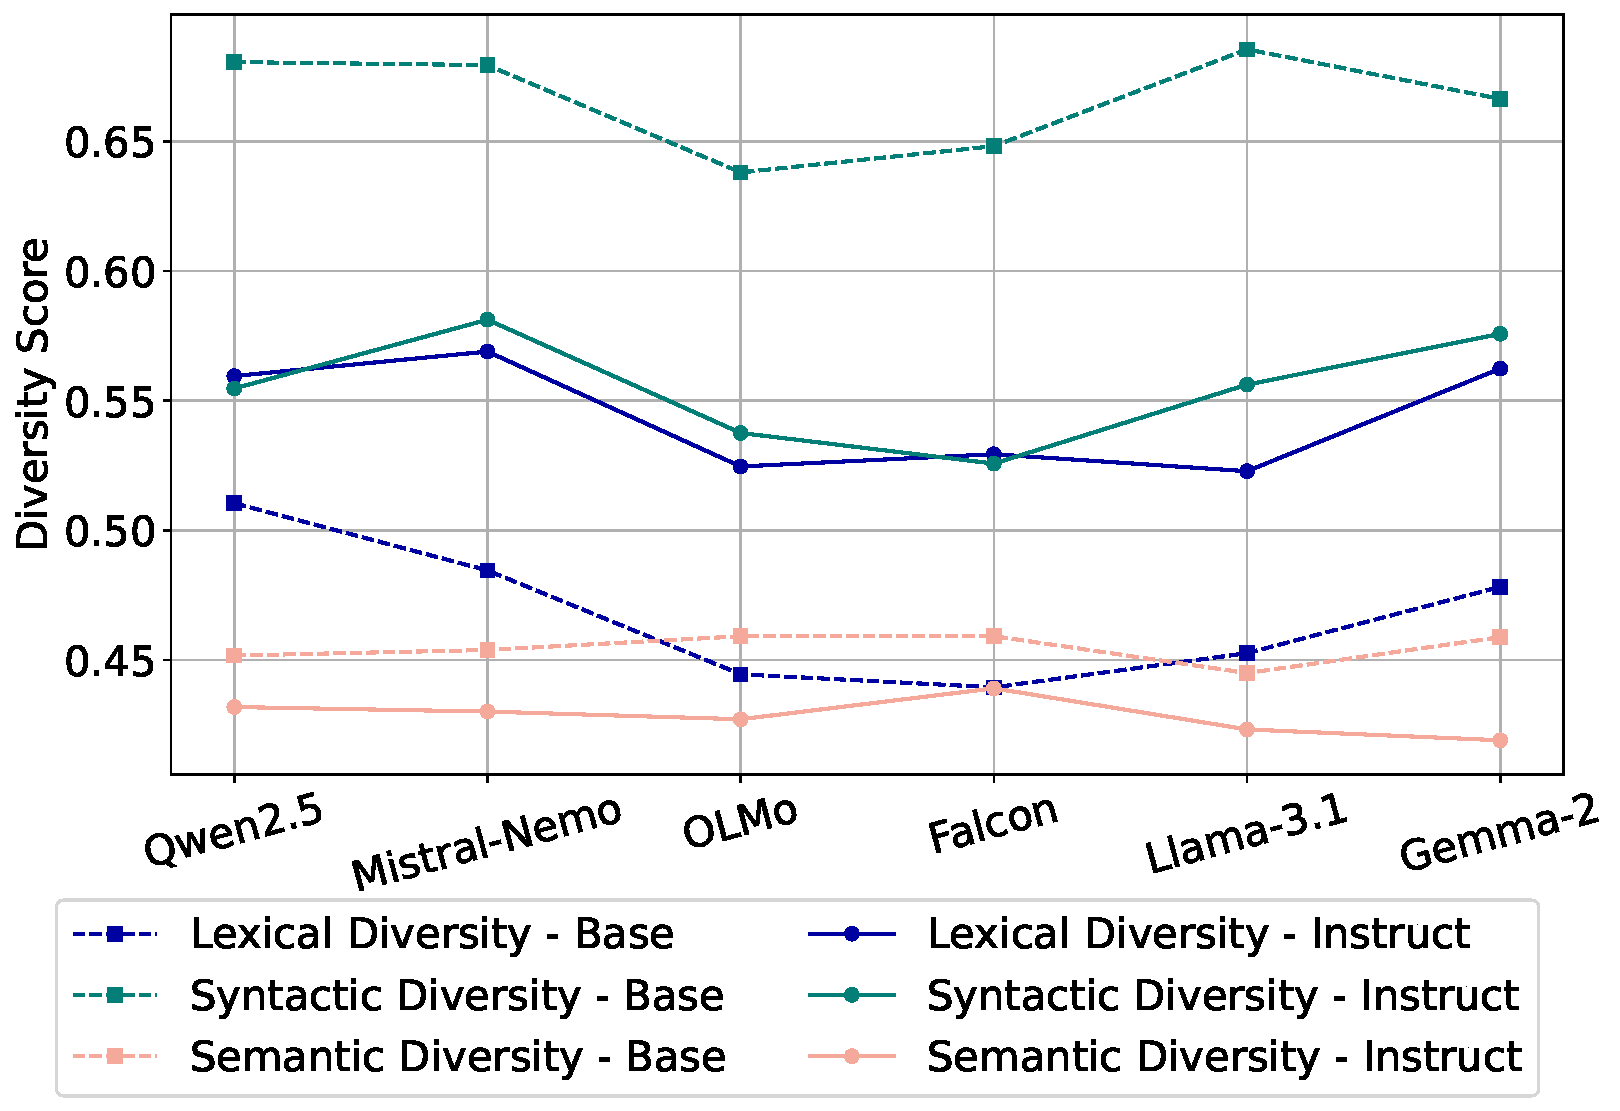
\includegraphics[width=0.9\columnwidth]{figures/base_instruct.pdf}
    \caption{Impact of instruction tuning.}
    %Experiments are conducted on the story generation task.
    \label{fig:base}
\end{figure}

Furthermore, we note that, across most models, the relative ranking of diversity scores remains stable as the temperature varies. This suggests that conducting experiments with a fixed temperature is sufficient for consistent evaluation. Based on our findings, we set the temperature to 0.6 for all other experiments. Figure~\ref{fig:decoding} shows that at a temperature of 0.6, the relevance to prompts remains relatively high while diversity scores significantly improve compared to lower temperatures. In fact, the creators of Llama-3.1 \citep{dubey2024llama} also identified a temperature of 0.6 as achieving the optimal balance between creativity and coherence.



\subsection{Impact of Model Scale and Quantization}\label{sec:scale_quant}

The Qwen2.5 model has been released in various sizes, ranging from 0.5B to 72B parameters. Due to computational resource constraints, we limit our exploration of linguistic diversity to models up to 32B parameters. The results are presented in Figure \ref{fig:scale_quant}. \textit{We observe that lexical diversity consistently increases with model size, while semantic diversity remains stable throughout}. In contrast, syntactic diversity remains relatively stable overall but exhibits an initial increase followed by a decline, peaking at 7B parameters, indicating that scaling up is not always the solution to higher diversity.

%To do: try different quantization approaches (e.g. GPTQ)

\begin{figure}[t]
    \centering
    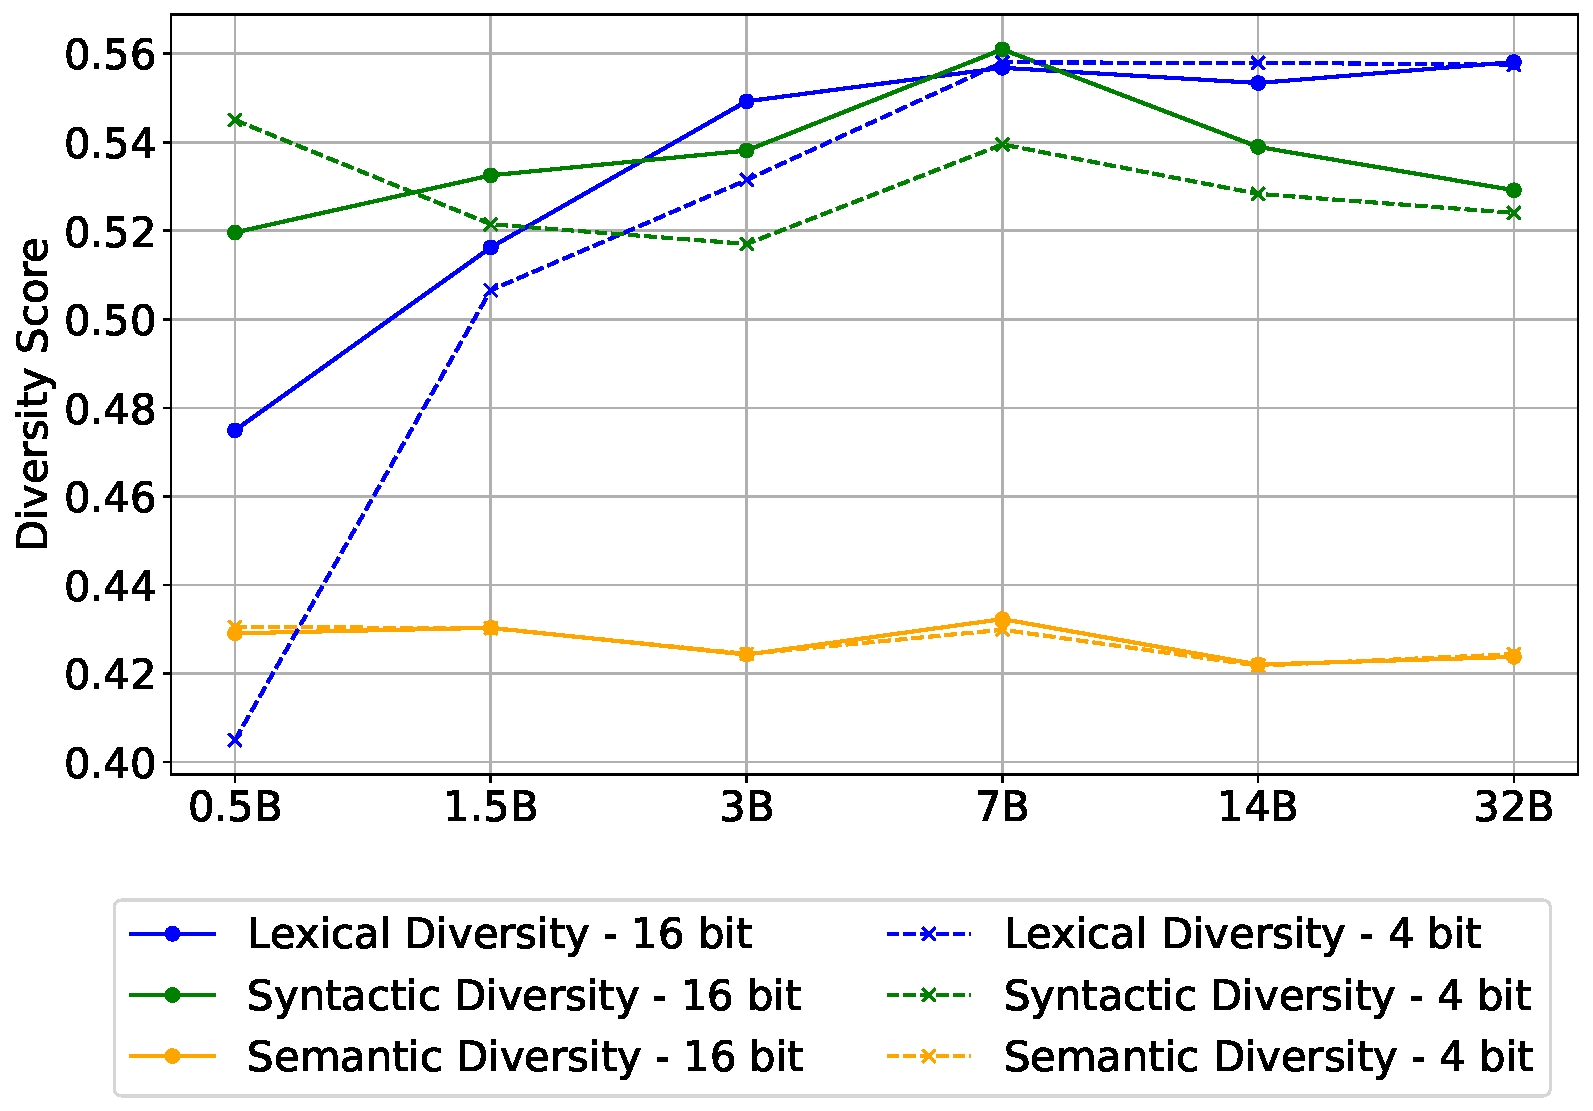
\includegraphics[width=0.9\columnwidth]{figures/scale_quant.pdf}
    \caption{Impact of model scale and quantization.}
    %Experiments are conducted with the Qwen2.5 series of models on the story generation task.
    \label{fig:scale_quant}
\end{figure}



We further investigate the impact of post-training quantization on linguistic diversity. 
%Utilizing the bitsandbytes library\footnote{\href{https://huggingface.co/docs/bitsandbytes/index}{https://huggingface.co/docs/bitsandbytes/index}}, 
We quantize the Qwen2.5 models of various scales to 4-bit precision with the bitsandbytes library\footnote{\href{https://huggingface.co/docs/bitsandbytes/index}{https://huggingface.co/docs/bitsandbytes/index}},
whereas the original models were run with bf16. As shown in Figure \ref{fig:scale_quant}, \textit{quantization does not affect semantic diversity but reduces both syntactic and lexical diversity}. The reduction in lexical diversity is more pronounced in smaller models, while the effect on syntactic diversity becomes more evident in larger models. This finding suggests that quantization has greater impact on the diversity of form rather than content.


\section{Conclusion}
Our study offers crucial insights into the linguistic diversity of current LLMs. By leveraging a comprehensive evaluation framework focused on lexical, syntactic, and semantic diversity, we provide a fresh perspective beyond traditional quality metrics. Our analysis reveals that, despite the impressive capabilities of LLMs in generating coherent and contextually appropriate text, there is a significant gap when it comes to replicating the linguistic richness characteristic of human language, especially for more creative tasks. Specifically, we observe that factors such as model scale, training data volume, and fine-tuning techniques critically influence diversity metrics.

These findings raise an important concern: as LLMs become more prevalent in content creation, their outputs may trend towards homogenization, risking a loss of linguistic richness. Notably, while instruction tuning improves lexical diversity, it constrains syntactic and semantic diversity, indicating a narrowing of expressive flexibility. Our research highlights the necessity of a more holistic and forward-looking approach in developing language models, one that prioritizes the preservation of linguistic diversity alongside optimizing performance metrics. We emphasize the need for novel strategies to balance the trade-offs between diversity and quality, ensuring that future models are capable of not only mimicking human language fluency but also maintaining its inherent diversity.

\section*{Acknowledgments}
We thank Professor Michalis Vazirgiannis for providing the computational resources that supported this project. This research was partially funded by the ANR-23-CE23-0033-01 SINNet project and the ANR-TSIA HELAS chair.


\bibliography{tacl2021, anthology}
\bibliographystyle{acl_natbib}

%\appendix
%\section{Benchmarked Models} \label{app1}
%\begin{table*}[h]
\small
\centering
\setlength{\tabcolsep}{1pt} %space between col
\renewcommand{\arraystretch}{1} %space between row
\scalebox{0.9}{
    \begin{tabular}{c|ccccccc}
    \toprule
    &  \textbf{Llama-3.1-8B}&  \textbf{Mistral-NeMo-12B}&  \textbf{Qwen2.5-7B}&  \textbf{Gemma-2-9b}&  \textbf{Falcon-7b}&  \textbf{OLMo-7B}\\
    \midrule
    \textbf{Organization}& Meta & Mistral & Alibaba & Google & TII & Ai2\\
    \textbf{Country}& USA & France & China & USA & UAE & USA\\
    \textbf{Open weights}& yes & yes & yes & yes & yes & yes\\
    \textbf{Open data}& no & no & no & no & partially & yes\\
    \textbf{Tokenization} & BPE (Tiktoken) & BPE (Tiktoken) & BPE & SentencePiece & BPE & BPE\\
    \textbf{Vocabulary size}& 128K & 128K & 151K & 256K & 65K & 50K\\
    \textbf{\#tokens}& 15T & unknown & 18T & 8T & 1.5T & 2.7T \\
    \textbf{Data filter}& \makecell{quality,\\ privacy, safety} & unknown & quality & \makecell{quality,\\ privacy, safety} & quality & \makecell{quality,\\ privacy, safety}\\
    \textbf{Synthetic data}& post-training & unknown & pre/post-training & post-training & unknown & post-training\\
    \textbf{Multilinguality}& yes & yes & \makecell{yes\\ (over 29 languages)} & not in particular & \makecell{yes\\ (Latin alphabet)}& no\\
    \textbf{Alignment}& \makecell{rejection sampling,\\ SFT, DPO} & SFT & SFT, DPO & SFT, PPO & SFT & SFT, DPO\\
    \textbf{Release date}& July 2024 & July 2024 & September 2024 & June 2024& May 2023 & February 2024\\
    \bottomrule
    \end{tabular}
}
    \caption{Comparison of benchmarked models.}
    \label{tab:models}

\end{table*}

\end{document}


%applications (dialogues, stories, summaries...), what (intoduction of diversity metrics by aspect), how (text-based evaluation metrics or model-based evaluation protocole), purpose (evaluate human written text, evalute LLMs, evaluate LLM checkpoints, evaluate promnpts, evaluate pretarining data), make a table of the applications, metrics and purposes


%protocole for prompting v.s. metric for evaluating text (unified approach)

%do llms need to produce diverse perspectives? what if it lowers coherence?

%foundation models should be able to adpat to different perspectives.

%Out of One, Many: Using Language Models to Simulate Human Samples

%Political Compass or Spinning Arrow?
Towards More Meaningful Evaluations for Values and Opinions in Large Language Models

%Improving Diversity of Demographic Representation in Large Language Models via Collective-Critiques and Self-Voting

%What Comes Next? Evaluating Uncertainty
in Neural Text Generators Against Human Production Variability

#Improving Diversity of Commonsense Generation by Large Language Models via In-Context Learning



%make table for different llms

#plot ngrams and syntactic structures that are the most frequent for each LLM (focus on the ones that are not common in human generated text)

Navigating the Grey Area: How Expressions of Uncertainty and Overconfidence Affect Language Models

Whose Opinions Do Language Models Reflect?

An Overview of Recent Approaches to Enable Diversity in Large Language Models through Aligning with Human Perspectives

Scaling Data Diversity for Fine-Tuning Language Models in Human Alignment

Scaling Data Diversity for Fine-Tuning Language Models in Human Alignment